\documentclass[10pt,letterpaper]{article}
\usepackage[margin=1in]{geometry}
\usepackage[T1]{fontenc}
\usepackage[utf8]{inputenc}
\usepackage{lmodern}
\usepackage{amsmath,amssymb}
\usepackage{booktabs,array,tabularx}
\usepackage{algorithm,algpseudocode}
\usepackage{graphicx,caption,microtype,needspace,float}
\usepackage{enumitem}
\usepackage[hidelinks]{hyperref}
\usepackage{url}
\setlength{\parindent}{0pt}
\setlength{\parskip}{5pt}
\setlength{\emergencystretch}{1em}
\setlist{itemsep=2pt,topsep=3pt}
\captionsetup{font=small,labelfont=bf}
\newcolumntype{L}{>{\raggedright\arraybackslash}X}
\newcommand{\R}{\mathbb{R}}
\newcommand{\E}{\mathbb{E}}
\newcommand{\ind}{\mathbf{1}}
\newcommand{\tr}{\operatorname{tr}}
\newcommand{\FDR}{\operatorname{FDR}}
\newcommand{\FDP}{\operatorname{FDP}}
\newcommand{\TPR}{\operatorname{TPR}}
\newcommand{\ISE}{\operatorname{ISE}}
\newcommand{\code}[1]{\nolinkurl{#1}}
\hypersetup{pdftitle={A Learned Variable Selector Built on IPSS},
 pdfsubject={The model with IPSS screening and a small MLP variable scorer}}
\begin{document}

\section{The Complete Procedure}\label{sec:overview}
The model takes $X\in\R^{n\times p}$, $y\in\R^n$, and a target FDR
$\alpha$, and returns a set of original columns of $X$. First, it keeps
variables selected by at least one of ten IPSS configurations at that target.
It then describes each retained variable with 443 measured or predicted numbers,
passes that vector through a small multilayer perceptron (MLP), and uses the
resulting scores to decide which candidates to select. The MLP has widths
$443\to128\to64\to1$. Its output estimates the chance that a variable is irrelevant.

There are two components fitted in advance. The fraction estimator $g$
uses XGBoost and describes how much signal the dataset may contain.
The variable scorer $F$ is the MLP. On a new dataset, both components
remain fixed; regressions and IPSS fits on that dataset supply their inputs.

The calculation has six steps. Screening uses both GB-IPSS and Lasso-IPSS
with each fixed $\delta\in\{-1,0,1,2,4\}$, giving ten final selection sets.
A variable passes if it belongs to any of these sets at the input target $\alpha$.
The four values $\{0,1,2,4\}$ also supply the existing MLP measurements;
$\delta=-1$ is used only for screening. The model does not predict an optimal
$\delta$. No reference datasets adjust its predictions on a new dataset.
The final selection is restricted to the variables that pass screening.

In the pseudocode, $a$ describes the dataset, $d$ summarizes
Lasso-IPSS, and $v_j$ describes column $j$ of $X$.

\begin{algorithm}[H]
\caption{Apply the model to a new dataset}\label{alg:model}
\small
\begin{algorithmic}[1]
\Require $X,y$, target $\alpha$, fitted $g,F$, saved input scaling, IPSS seed
\Ensure Selected set $\widehat S(\alpha)$
\State \textbf{Step 1.} Run GB-IPSS and Lasso-IPSS on $X,y$ with the seed.
\State For each method, calculate EFP scores and q-values at $\delta\in\{-1,0,1,2,4\}$.
\State \textbf{Step 2.} Set $s_j\gets\min_{m\in\{\mathrm{GB},\mathrm{Lasso}\},\,\delta}q_{j,m,\delta}$.
\State Keep candidates $C_\alpha\gets\{j:s_j\le\alpha\}$; return $\varnothing$ if this set is empty.
\State \textbf{Step 3.} From the full $X,y$, calculate $a\in\R^{302}$, $d\in\R^9$ and $v_j\in\R^{130}$.
\State \textbf{Step 4.} Apply $g$ to $a$; obtain $\widehat\pi$ and $\widehat t$ as in Section~\ref{sec:fraction}.
\State \textbf{Step 5.} Form shared vector $c\gets(a,\widehat t,\widehat\pi,d)\in\R^{313}$.
\For{$j\in C_\alpha$}
  \State Form $u_j\gets(c,v_j)\in\R^{443}$ and apply the saved input transformation.
  \State Pass it through layers $443\to128\to64\to1$ and a sigmoid to obtain $\widehat\eta_j$.
\EndFor
\State \textbf{Step 6.} Sort the candidates by increasing $\widehat\eta_j$.
\State Let $\mathcal K$ contain the positions at the ends of equal-score groups within $C_\alpha$.
\State For $k\in\mathcal K$, calculate $\widehat r_{k,\alpha}\gets k^{-1}\sum_{\ell=1}^k\widehat\eta_{(\ell;\alpha)}$.
\State $k^*\gets\max\bigl(\{0\}\cup\{k\in\mathcal K:\widehat r_{k,\alpha}\le\alpha\}\bigr)$.
\State \Return The first $k^*$ candidates in the sorted order.
\end{algorithmic}
\end{algorithm}

The following sections explain these six steps, the fitted components,
and the model's measured performance.

\section{The Six Steps in Detail}
\subsection{Step 1: Calculate IPSS measurements}\label{sec:ipss}
IPSS supplies measurements of how consistently a variable is selected
when the data are repeatedly split. The model uses gradient boosting
(GB), which scores variables by tree importance, and Lasso, which
selects nonzero regression coefficients. These fits predict $y$ on
the given dataset; they are separate from the components $g$ and $F$
trained in advance.

For each random split, fit the base method on two disjoint halves
of the observations. GB uses 100 splits, giving 200 half-sample fits;
Lasso uses 50 splits, giving 100 fits. At a threshold $\lambda$,
average the indicators of whether a fit selects variable $j$:
\[
 P_j(\lambda)=\frac{1}{2B}\sum_{b=1}^{2B}
 \ind\{\text{fit }b\text{ selects }j\text{ at }\lambda\}.
\]
For GB, $\lambda$ is an importance cutoff; for Lasso, it is a penalty.
If 150 of the 200 GB fits select a variable, its frequency is 0.75.
The frequencies across thresholds form its \emph{stability path}.
They describe repeated selections, not the probability of relevance.

The IPSS routine \cite{ipss,ipssgb} combines each path into an EFP
(expected false positives) score. Lower scores indicate stronger
evidence. EFP can exceed one; it is not the probability of irrelevance
estimated by $F$. The parameter $\delta$ changes the weighting of thresholds
in this calculation. Evaluate $\delta=-1,0,1,2,4$ on each of the two
stored paths, obtaining ten score vectors. The half-sample fits are reused
across these choices. The eight vectors at $\delta=0,1,2,4$ supply the
original measurements, while all ten are available to the screening step.
No optimal $\delta$ is predicted.

\textbf{How a path becomes a score.} Each threshold produces one
frequency $P_j(\lambda)$. IPSS first replaces it by
\[
 h_r(P)=\{\max(2P-1,0)\}^{r},\qquad
 r=3\text{ for GB},\quad r=2\text{ for Lasso}.
\]
Frequencies at or below one half contribute zero. Larger frequencies
contribute more, so repeated selection matters more than an occasional
selection. For example, $P=0.75$ contributes $0.125$ for GB and $0.25$
for Lasso. These powers are the fixed choices of the IPSS routine, not
quantities learned by the MLP.

The routine combines these contributions across thresholds by numerical
integration, rather than selecting one threshold. The weights correspond
to a measure proportional to $\lambda^{-\delta}d\lambda$: changing $\delta$
changes the relative emphasis on stricter and more permissive thresholds.
The four original choices give the MLP several summaries of the same path;
$\delta=-1$ supplies one additional screening configuration per method.
Let $A_{j,\delta}$ denote the integrated contribution for variable $j$.

IPSS also integrates a bound expression using the average number of columns
selected by the half-sample fits and the number of splits; denote that
quantity by $I_\delta$. Selecting many columns makes accidental repeated
selection easier, and increases the bound expression. The library stops
its bound accumulation before the next addition would exceed $0.05$,
then integrates the variable contributions over the retained thresholds.
The numerical normalization is recomputed for that retained range.
If the branch uses $m$ columns internally, the stored EFP score before
mapping back to all original columns is
\[
 E_{j,\delta}=\frac{I_\delta}
 {\max\{A_{j,\delta},I_\delta/m\}},
\]
rounded to eight decimal places. Thus stronger repeated-selection evidence
reduces the score, whereas the denominator floor limits it to $m$.
When $m<p$, scores at least $m-1$, together with omitted columns, are
represented by the uninformative value $p$. This is a convention for the
input measurement. The explicit candidate rule is given in Step~2.

The implementation uses IPSS 1.1.11. GB half-sample fits have 100 depth-one
trees and up to 100 importance thresholds; Lasso uses up to 25 penalties.
The IPSS routines also shorten a path after it stops changing. The exact
integration and bound expressions are retained in the installed IPSS
routine and \code{explore/paths.py}. They are not refitted by the model.
The target FDR $\alpha$ is used in the candidate rule in Step~2 and the final rule in Step~6. The theoretical assumptions
behind IPSS do not, by themselves, supply a guarantee for the later learned
scores and their cumulative averages.

\textbf{IPSS's internal column reduction.} This reduces the cost of
its repeated fits. For a continuous response, the Lasso branch makes three
bootstrap samples, fits a preliminary Lasso on each, and sums the absolute
coefficients for every column. It retains the top $\min(p,200)$ columns.
For a binary response, this branch uses penalized logistic regression.
The preliminary penalty is set from the observed correlations, as implemented
in IPSS; it does not use the final target $\alpha$.

The GB branch fits three preliminary ensembles of 50 depth-one trees and
adds their gain importances. If $r$ columns have positive total importance,
it retains those columns and randomly fills the set to
$\min\{p,\max(100,\lfloor1.5r\rfloor)\}$ columns. This random fill deliberately
allows some columns with zero preliminary importance to enter the repeated
fits. These preliminary fits occur before the half-sample fits described
above.

Results are mapped back to all $p$ original columns: a column omitted by
one IPSS branch receives EFP score $p$ and zero frequency summaries for
that branch. Its other measurements are still computed using the full $X,y$.
This internal reduction and the next screening step have different roles:
internal reduction determines which columns receive each branch's path fits;
Step~2 determines which original columns may enter the final selection.
Step~1 supplies ten EFP vectors and two frequency tables, all indexed by the
original columns. A column omitted by both branches cannot pass the screen
at the targets plotted here.

\subsection{Step 2: Keep variables selected by any of ten IPSS configurations}\label{sec:screen}
For method $m$ and weighting value $\delta$, convert its EFP scores to
IPSS q-values. For a particular score vector $E$, the conversion is
\[
 q_j=\min_{t\ge E_j}\frac{t}{|\{k:E_k\le t\}|},
\]
where $t$ runs over distinct scores. Tied scores use the size of the full
tied group. At target $\alpha$, that IPSS configuration selects
$S_{m,\delta}(\alpha)=\{j:q_{j,m,\delta}\le\alpha\}$. Define
\[
 C_\alpha=\bigcup_{m\in\{\mathrm{GB},\mathrm{Lasso}\}}
           \ \bigcup_{\delta\in\{-1,0,1,2,4\}}S_{m,\delta}(\alpha).
\]
Equivalently, compute $s_j=\min_{m,\delta}q_{j,m,\delta}$ once and keep
$j$ when $s_j\le\alpha$. The union uses the final IPSS selections at the
same target as the model. It does not keep every variable selected in any
individual half-sample fit. The ten configurations reuse two stored paths;
they do not require ten new collections of repeated fits.

For example, at $\alpha=0.10$, a variable with ten q-values all above
$0.10$ is excluded, even if the MLP would give it a favorable score.
A variable with at least one q-value at or below $0.10$ proceeds to the MLP.
It is still only a candidate: Step~6 may exclude it. An empty union produces
an empty final selection.

The purpose is to require some IPSS evidence before allowing the learned
scorer to select a variable. The cost is that a truly relevant variable
missed by all ten configurations cannot be recovered later. The union itself
has no established FDR bound at $\alpha$, and neither does the full learned
procedure merely because it uses this screen. The evaluation measures both
loss of true discoveries and changes in false discoveries.

\subsection{Step 3: Calculate the input measurements}\label{sec:inputs}
From $X$, $y$, and the two IPSS results, calculate three sets of
numbers: $v_j\in\R^{130}$ for each of the $p$ variables, $a\in\R^{302}$
for the dataset, and $d\in\R^9$ for the additional Lasso-IPSS
summaries. These are calculated statistics, not learned outputs.
The true relevant variables, their number, and simulation parameters
are not supplied. Regressions fitted within this step calculate
measurements; they do not retrain $g$ or $F$.

\subsubsection{What is measured, and what is learned}
A column $X_j$ contains $n$ observed values. The model does not feed
that entire column directly to $F$. Instead, it describes the column
using the fixed measurements below: correlations, regression results,
and IPSS summaries. The formulas defining the measurements are chosen
in advance. Training learns how to combine their values into a score.

The measurements use the full observed $X$, including columns that did
not pass screening. Only candidates receive an MLP prediction. For example, the correlations for variable $j$
are calculated against all other predictors. The regressions below
also use the full predictor matrix. The additional
regressions in this step are fitted for these measurements; they are
not the half-sample fits previously used by IPSS.

\subsubsection{Measurements for each variable}
These measurements describe how column $j$ relates to $y$, how that
relationship changes when other predictors are included, and what
IPSS reports about it.
\begin{center}\small
\begin{tabularx}{\linewidth}{Lr}
\toprule
Measurements for one variable & Number\\
\midrule
Correlations with other columns of $X$ & 5\\
Correlations with $y$ and ridge-regression results & 28\\
GB-IPSS scores and selection frequencies & 17\\
Ridge-regression results with a smaller penalty & 8\\
Unpenalized regression coefficients and uncertainty measures & 16\\
Lasso coefficients and adjustments using its residuals & 24\\
Regression results after applying $\tanh$ to the columns & 15\\
Lasso-IPSS scores and selection frequencies & 17\\
\midrule
Total & 130\\
\bottomrule
\end{tabularx}
\end{center}

\textbf{Transformations.} Standardize each nonconstant column of $X$ and $y$
to mean zero and variance one, using denominator $n$. Then make
four versions of the predictor matrix by applying
\[
 h(u)=u,\qquad u^2,\qquad e^{-u^2/2},\qquad\sin(2u),
\]
and standardizing the transformed columns again. Denote each resulting
matrix by $Z$ and the standardized response by $\widetilde y$.
Constant columns are represented by zeros; numerical denominators have a
small positive floor in the implementation.
For example, $u^2$ can reveal a relationship that is strong at large
positive and negative values even when ordinary correlation is small.
All four transformations are used on every dataset.

\textbf{Correlations.} For column $j$, record the maximum and mean
absolute correlation with other predictors, the sum of squared
correlations, and the fractions exceeding 0.5 and 0.8 in absolute
value. Set self-correlation to zero and divide means and fractions
by $p$. Its absolute correlation with $y$ under a transformation is
$|Z_j^\top\widetilde y|/n$.

\textbf{Ridge regression.} Correlation with $y$ alone can favor a
variable merely because it correlates with a relevant predictor.
Regressing $y$ on all columns together provides additional information.
Ridge regression keeps the calculation possible with many correlated
predictors. Its coefficient vector is
\[
 \widehat\beta_\lambda=(Z^\top Z+\lambda I)^{-1}Z^\top\widetilde y.
\]
For each coefficient, record its magnitude and that magnitude divided
by an estimated standard error. The latter measures coefficient size
relative to estimated uncertainty. Use three penalties,
$\lambda=\max(n,p)\{0.01,0.1,1\}$. Three pairs plus one correlation
with $y$ give seven numbers per transformation, or 28 total. An extra
pair per transformation gives eight more numbers, using penalty
$\max(n,p)10^{-4}$ if $p\le0.75(n-1)$, and $0.01\max(n,p)$ otherwise.

\textbf{Unpenalized regression.} When
$n-p-1\ge\max(15,0.1n)$ and the transformed columns are linearly
independent, also fit ordinary least squares (OLS). Each transformation
supplies four numbers: absolute coefficient, absolute $t$ statistic,
a version of that statistic allowing unequal residual variances
(HC3), and negative log two-sided $t$-tail probability. Otherwise,
use zeros and indicators that the fit was unavailable. These are
predictive inputs, not separate tests used to select variables.

\textbf{Lasso and its remaining errors.} For each transformation,
fit Lasso using five-fold cross-validation over 40 penalties. The folds
split the observations of this dataset. Keep
coefficients from the lowest-error fit and from a more strongly
penalized fit whose error is within one estimated standard error
of the minimum. Let $b$ be the latter coefficients and
$e=\widetilde y-Zb$ its residual.

To measure association with the remaining response, one adjusted
coefficient is $b+Z^\top e/n$; another is
$b+MZ^\top e/n$, where $M$ accounts for correlations among predictors.
Specifically, set $H=Z^\top Z/n$ and $M_0=(H+0.1I)^{-1}$, then divide
row $j$ of $M_0$ by $(M_0H)_{jj}$. Retain the two original coefficient
magnitudes and each adjusted magnitude and its ratio to estimated standard error: six numbers per transformation, or 24 total.

\textbf{Additional nonlinear measurements.} Applying $\tanh$ to a
predictor captures relationships that flatten at large positive or
negative values. Fifteen numbers come from Lasso, OLS, and the
residual-based adjustments above. Some adjustments use all predictors;
others use only the 5 or 10 strongest correlated neighbors, requiring
absolute correlation above 0.5 and retaining boundary ties. The
latter also record how many neighbors were used.

\textbf{IPSS measurements.} Each run supplies 17 numbers. At each
of the four $\delta$ values, record log EFP, the IPSS q-value, and the
fraction of variables with EFP no larger than variable $j$'s. The
remaining five summarize its selection frequencies $P_j$: maximum,
mean, fraction above 0.5, fraction above 0.8, and mean of
$(\max(2P_j-1,0))^2$. This last squared-frequency summary is an
input measurement for both methods; it is separate from the cubic
transformation used to calculate GB's EFP scores in Step~1.
For clarity, an IPSS q-value is calculated from the EFP scores by
\[
 q_j=\min_{t\ge E_j}\frac{t}{|\{k:E_k\le t\}|},
\]
where $t$ runs over the distinct scores. This q-value is an input
measurement. The model's score in Step~5 supplies the final order among candidates.

\subsubsection{Measurements for the dataset}
The dataset measurements describe the conditions in which a variable
is evaluated. At this step, they contain no predictions from the
fitted components.
The 302 entries used by the first component comprise 64 basic
summaries of dimensions, correlations, associations, and ridge fits;
124 summaries of additional regression fits; 104 summaries describing
how strong and widespread the variable measurements are; nine
summaries of GB-IPSS; and one indicator identifying GB as the main
IPSS result. The summaries include means, standard
deviations, quantiles, maxima, and indicators of unavailable fits.
For example, the basic entries include $\log n$, $\log p$, $p/n$,
summaries of the correlation matrix and its eigenvalues, and fourth moments
of $X$ and $y$. Associations with $y$ are summarized for the four
transformations above and for rank-transformed predictor columns.
Cross-validated ridge prediction errors describe which response patterns
are easy to predict. The regression and variable-score summaries describe
whether apparently strong evidence is isolated or widespread.

Each IPSS run supplies nine dataset summaries: the fraction retained
by its preliminary step, path length, default $\delta$, and six
summaries of maximum selection frequencies. The GB summaries are
already included in $a$; store the nine Lasso summaries separately
as $d$. Internal cross-validation uses
five shuffled folds with seed 417; these scores describe the dataset
rather than test the final model. The exact input order is in the retained schema
\code{models/expanded_f.json}; calculations, including standard errors
and numerical safeguards, are in \code{explore/}.

\subsection{Step 4: Estimate the relevant fraction}\label{sec:fraction}
The first fitted component $g$ uses the 302 dataset measurements
$a$ to estimate how many of the $p$ variables are relevant. It
contains 250 trees, each with maximum depth three. Its output is
restricted to $[-7,3]$ and converted to a fraction:
\[
 \widehat t=\max(-7,\min(3,g(a))),\qquad
 \widehat\pi=\frac{1}{1+e^{-\widehat t}}.
\]
For $p=300$, $\widehat\pi=0.10$ estimates 30 relevant variables
overall. It does not identify them or instruct the model to select
exactly 30. The denominator is the original $p$, not $|C_\alpha|$.
The estimate provides context for the next component.
Both $\widehat t$ and $\widehat\pi$ are retained as inputs; they are
two representations of the same estimate.

\subsection{Step 5: Score the candidate variables}\label{sec:score}
Combine the dataset measurements, fraction estimate, and additional
Lasso-IPSS summaries into a vector shared by all columns:
$c=(a,\widehat t,\widehat\pi,d)\in\R^{313}$. For each $j\in C_\alpha$,
attach its 130 variable measurements:
\begin{equation}\label{eq:input}
 u_j=(\underbrace{c}_{313\text{ shared entries}},
       \underbrace{v_j}_{130\text{ variable entries}})\in\R^{443}.
\end{equation}
For $p=300$ and $|C_\alpha|=40$, the MLP receives 40 rows of 443 entries.
The dataset summaries and each row's measurements were still calculated
using all 300 original columns. The same fitted MLP is applied to the
40 candidate rows, using the same weights.
There are two operations within this step: rescale the inputs, then apply
the network.

\textbf{Input transformation.} For coordinate $q=1,\ldots,443$, calculate
\[
 T(u_{jq})=\operatorname{sign}(u_{jq})\log(1+|u_{jq}|),\qquad
 \widetilde u_{jq}=\operatorname{clip}
 \left(\frac{T(u_{jq})-\mu_q}{s_q},-10,10\right).
\]
The constants $\mu_q,s_q$ are the weighted mean and standard deviation of
that transformed coordinate in the training rows; $s_q$ is bounded below
by $0.001$. They are saved with the model. The logarithm reduces differences
in scale between measurements, and clipping limits extreme inputs.
These constants are not estimated again on a new dataset. This operation
is separate from transforming columns of $X$ to calculate the measurements
in Step~3.

\textbf{Two hidden layers and one output.} At application time, calculate
\begin{align*}
 e_j^{(1)}&=\operatorname{GELU}(W_1\widetilde u_j+b_1)\in\R^{128},\\
 e_j&=\operatorname{GELU}(W_2e_j^{(1)}+b_2)\in\R^{64},\\
 \ell_j&=w_3^\top e_j+b_3,\qquad
 \widehat\eta_j=F(u_j)=\frac{1}{1+e^{-\ell_j}}.
\end{align*}
Here $W_1$ is $128\times443$ and $W_2$ is $64\times128$.
GELU is the fixed nonlinear function $z\Phi(z)$, where $\Phi$ is the
standard normal distribution function; it is applied to each coordinate.
All matrix entries and biases are learned during training. Together they
contain 65,153 fitted parameters.

The 443-entry vector consists mostly of measurements with specified
formulas, plus the outputs of $g$. The 64-entry vector $e_j$ is a learned
representation: its coordinates are combinations that the network finds
useful for predicting relevance. Its individual coordinates are not assigned
names such as ``correlation'' or ``stability.'' The final linear layer and
sigmoid turn this representation into one score. A score of $0.02$ is an
estimated $2\%$ chance of irrelevance, not an independently validated
probability. All variables use the same network, while the shared entries
allow its predictions to depend on the dataset.

During training, dropout independently sets a hidden-layer output to zero
with probability $0.05$ and rescales the retained outputs by $1/0.95$.
Dropout is applied after each GELU layer. It is switched off when selecting
variables, so repeated scoring of identical inputs gives the same result.
Every candidate now has one score. The target $\alpha$ determined which
variables passed the screen; it is not an input to the MLP. A variable's
measurements and score do not change when $\alpha$ changes. For several
requested targets, the implementation scores the union of their candidates
once and reuses the scores.

\subsection{Step 6: Order and select the candidates}\label{sec:selection}
Sort only the variables in $C_\alpha$ by increasing score, writing
$(k;\alpha)$ for the original column at position $k$ in this candidate order.
Average the first $k$ candidate scores:
\begin{equation}\label{eq:average}
 \widehat r_{k,\alpha}=\frac{1}{k}\sum_{\ell=1}^k\widehat\eta_{(\ell;\alpha)}.
\end{equation}
Choose the largest $k\le|C_\alpha|$ with $\widehat r_{k,\alpha}\le\alpha$,
including or excluding identical scores together. If no allowed $k$ qualifies,
select nothing. Recompute these averages inside the candidate set; merely
intersecting an unscreened final selection with $C_\alpha$ gives a different rule.
For illustration, suppose all four following variables pass screening at
both targets considered below:
\begin{center}\small
\begin{tabular}{lrr}
\toprule
Variable & Predicted chance of irrelevance & Average so far\\
\midrule
$X_3$ & 0.01 & 0.0100\\
$X_2$ & 0.02 & 0.0150\\
$X_1$ & 0.06 & 0.0300\\
$X_4$ & 0.30 & 0.0975\\
\bottomrule
\end{tabular}
\end{center}
At $\alpha=0.05$, select $X_3,X_2,X_1$. At $\alpha=0.10$, select
all four. A variable's own score may exceed $\alpha$; the rule uses
the average score. Ties enter together so the result does not depend
on an arbitrary ordering of equal scores.

Within a fixed candidate set, the running averages cannot decrease as
more candidates are included. However, changing $\alpha$ also changes
$C_\alpha$, so the final selections need not be nested across targets.
For example, admitting more candidates can change the average at the
position of a previously selected variable, even though its own score stays fixed.
If the scores equaled probabilities of irrelevance conditional on all
information used to choose the set, their average would equal its conditional
expected FDP. Estimated scores do not provide that guarantee; screening
does not remove this limitation.


\section{Fitting the Model}\label{sec:training}
\subsection{Training data and labels}
The model uses 5,216 synthetic fitting datasets from 564 settings: 3,296
datasets from 324 original settings and 1,920 datasets from 240 additional
settings. Every original variable supplies one row, giving 1,636,538 rows
with 443 entries each. For dataset $i$, let $S_i$ be its known relevant set.
The fitting label is $z_{ij}=\ind\{j\notin S_i\}$: zero for a relevant
variable and one for an irrelevant variable. The true set is used for
this label, never to construct an input row. All rows remain in training;
the screen restricts selection when the fitted model is applied.

The original data have Gaussian predictors with Toeplitz, block or
shared-factor dependence, additive transformed responses and Gaussian
noise, with $60\le n\le400$ and $30\le p\le600$.
The added data span $40\le n\le1000$, $8\le p\le4000$ and 0--80
relevant variables. They include Gaussian, heavy-tailed, lognormal,
binary, ordinal and mixture predictors; several correlation structures,
including nearly duplicate columns; and linear, nonlinear, interaction,
binary, count and null responses. Continuous-response noise can be
Gaussian, heavy-tailed, heteroskedastic or contaminated, with SNR between
approximately 0.2 and 4. These are fixed sampled settings, not every
combination of the listed choices. Neither component is fitted using a
real predictor matrix.

\subsection{Fit the fraction estimator and construct its training predictions}
The fraction estimator $g$ retains its fit on the 3,296 original datasets.
Each dataset supplies two records, exchanging GB and Lasso as the main
IPSS method, for 6,592 records. Its training target is the log odds of
the relevant fraction, clipping that fraction to $[0.001,0.999]$ before
taking log odds. The loss is squared error with equal total weight per
setting. The retained XGBoost regressor has 250 trees, maximum depth 3,
learning rate $0.035$, minimum child weight 20 and leaf penalty 30;
row and column sampling fractions are $0.85$ and $0.90$.

To construct the MLP's inputs on the original data, divide the 324 settings
into the same five groups used in fitting $g$. Fit a temporary copy of $g$
on four groups and predict the fifth. All datasets and both IPSS records
from a setting remain together. Keep the GB-main prediction, clip it to
$[-7,3]$, and include that value and its sigmoid in the input row. For the
additional 1,920 datasets, use the retained $g$, which was never fitted on
those datasets. Thus the MLP learns from predicted fractions rather than
being given the true fraction. Application uses only the retained $g$;
the temporary copies are not part of the deployed model.


\subsection{Fit the MLP}
Training has two stages. First, initialize the network by fitting weighted
binary log loss with equal total weight per setting, equal weight per
dataset within a setting, and equal weight per variable within a dataset.
For setting $s$ with $M_s$ datasets and dataset $i$ with $p_i$ columns,
the initial row weight is proportional to $1/(M_sp_i)$. The input means
and standard deviations in Step~5 are computed with these weights on
the fitting rows and retained throughout both stages. AdamW uses initial
learning rate $10^{-3}$, weight decay $10^{-4}$, batches of 8,192 rows,
dropout 0.05 and gradient norm limit 10. The learning rate decreases to
$5\times10^{-5}$ over 35 epochs. The initialization checkpoint is epoch 1,
which minimizes weighted log loss on the 600 broad validation datasets.
The initial random seed is 2026110518.

The second stage concentrates more training weight on variables that
IPSS considers plausible. The aim is to spend more of the fit separating
the variables that may actually enter the final candidate set. For each
training variable, take the minimum of its eight IPSS q-values from
GB and Lasso at $\delta=0,1,2,4$. Assign multiplier
\[
 a_{ij}=\begin{cases}10,&\min_{m,\delta\in\{0,1,2,4\}}q_{ij,m,\delta}\le0.5,\\
 1,&\text{otherwise}.\end{cases}
\]
Within each dataset, renormalize these multipliers so its total weight
is unchanged. Next, rescale the original-data rows to receive 65\% of
the total weight and the added-data rows to receive 35\%. Settings within
each source still have equal total weight. Finally, rescale all row
weights to mean one. Both relevant and irrelevant variables receive the
same multiplier rule; no additional class weight is used.
The threshold 0.5 is a training-weight choice. At application, screening
still uses the requested $\alpha$ and all ten configurations, as in Step~2.

With these weights, continue to minimize
\[
 \mathcal L=-\frac{1}{N_{\rm rows}}\sum_{i,j}w_{ij}
 \{z_{ij}\log\widehat\eta_{ij}+(1-z_{ij})\log(1-\widehat\eta_{ij})\}.
\]
Only the 65,153 MLP parameters are updated. The fraction estimator,
measurement formulas, input scaling and final selection rule remain fixed.
The second stage has the following settings:
\begin{center}\small
\begin{tabular}{ll}\toprule
Choice & Value\\\midrule
Network & $443\to128\to64\to1$, GELU, training dropout 0.05\\
Optimizer & AdamW; weight decay $10^{-4}$\\
Learning rate & $3\times10^{-4}$, cosine decrease to $1.5\times10^{-5}$ over 20 epochs\\
Batch size / gradient norm limit & 8,192 / 10\\
Random seed & 2026110555\\
Checkpoint retained & Epoch 5 of the second stage\\\bottomrule
\end{tabular}\end{center}

\subsection{Choose the fitted checkpoint}
Checkpoint selection explicitly checks whether the model preserves
the original standard-benchmark performance. It uses 500 previously
examined standard datasets (10 per setting), plus 1,360 previously
examined validation datasets: 600 broad draws and 380 draws at each of
two additional validation difficulties. These are development data.
Their labels do not enter gradient updates, but their results guide the
choice of training configuration and checkpoint.

At each of $\alpha=0.05,0.10,0.20$, screen checkpoints using minimum-TPR
requirements fixed from earlier development results. Apply these requirements
to the standard, broad nonnull, easier synthetic, easier real-predictor,
harder synthetic and harder real-predictor groups. Each group, including
null groups, must have mean FDR at most $\alpha+0.02$. Among passing
checkpoints, maximize mean TPR over the harder synthetic and harder
real-predictor groups and the three targets, subject to the recorded
minimum-improvement requirement. The archived training protocol and
selection records retain the numerical thresholds. Six training
configurations were compared; the weighting described above was the only
one passing these requirements.

Before fixing the final checkpoint, check all 9,310 old benchmark datasets.
Apply the recorded minimum-TPR requirements separately to the standard,
stress, challenge and replication groups, with mean FDR at most
$\alpha+0.02$ at the three targets. The chosen model passes these checks.
These are empirical development requirements, not a claim of FDR control.
The model remains frozen for the new evaluation below. No training or
model selection uses these new evaluation outcomes.

\textbf{Application.} The public call
\code{explore.current.select_features(X,y,targets=[0.05,0.1,0.2])}
returns original column indices numbered from zero, together with
candidate counts and final selection counts for each target.
The current release is recorded in \code{models/active_model.json};
the MLP weights and input scaling are in
\code{models/retained_mlp_hard_rows.pt}. Application loads one MLP and
the fraction estimator, without training or evaluation datasets.
There is no second variable scorer $H$ or correction from reference datasets.






\section{Evaluation}\label{sec:experiments}
The evaluation focuses on limited sample size relative to the number of variables.
For every dataset, draw
\[
 U\sim\mathrm{Uniform}(\log50,\log500),\qquad
 p=\operatorname{round}(\exp U),
\]
and use either $n=p$ or $n=\max\{50,\lfloor0.8p\rfloor\}$.
Thus $50\le n\le p\le500$. There are 40 prespecified combinations of
data source, response rule and sample-size regime, with 100 new datasets
per combination, for 4,000 datasets in total. The original 28 combinations
contribute 2,800 datasets, and a subsequent addition of 12 combinations
contributes 1,200 datasets. Each batch's dimensions, random seeds,
generators and model files were fixed before measuring that batch's performance.
All settings and all repetitions are reported; none are selected for a
favorable result. The model is not refitted for this evaluation.

The first eight figures use Gaussian and RNA-seq designs based on
\cite{ipssgb}, with the dimensions above and the data generation specified
below. The appendix adds
simple synthetic responses, two standard synthetic benchmark families,
and five additional real predictor sources. The two added synthetic
families are sparse correlated-Gaussian linear regression and Friedman \#1;
the two added real sources are MNIST and BASEHOCK.
Some predictor distributions and response functions overlap fitting.
The study measures small-sample selection performance, rather than
assuming that every response mechanism is new to the model.

\subsection{Comparisons and averaging}
Compare the model with GB-IPSS, Lasso-IPSS and LassoCV. Every method
receives the same $X,y$ within a draw. The two IPSS baselines share their
stability paths with the model. GB-IPSS uses $\delta=1.25$ for continuous
responses and $\delta=1$ for binary responses, matching Table S1 of
\cite{ipssgb}. Lasso-IPSS uses its default correlation rule: setting
self-correlations to zero, let $a$ be the mean absolute correlation over
all $p^2$ entries and $b$ the mean columnwise maximum. Its $\delta$ is 1
if $a\le0.05$, 0 if $a\ge0.25$, and
$\operatorname{clip}(2.25-5a-2b,0,1)$ otherwise. LassoCV selects the
nonzero coefficients of the model's linear LassoCV measurement, with
five-fold prediction-error selection; it also treats binary $y$ as numeric
0/1 and has no target-FDR input. These comparisons use the retained
implementation of these methods, not all methods from the original paper.

Targets are $\alpha=0,0.01,\ldots,0.50$. Within each setting, average
realized FDP and TPR over the 100 datasets. Where a figure combines the
two sample-size regimes, give each regime equal weight. The left panel
shows empirical FDR and the right panel shows TPR, with the full target
range displayed. Real-predictor experiments repeatedly sample fixed
observed matrices and generate new responses; they are not independent
collections of new patients, speakers, subjects or objects. Their truth
is the planted response support. Predictive proxies are counted as false
selections when they are outside that support. No general FDR guarantee
is asserted for the learned selection rule.

The curves are Monte Carlo means; per-setting standard errors are retained
with the numeric results. All 4,000 inputs are regenerated and checked
against their saved hashes, and TP/FP counts are recounted from the saved
selected sets. The model's selection rule is independently reconstructed
for every target and dataset. The public application interface is also
checked on one dataset per setting using the saved IPSS paths. The data
generators and frozen draws are retained in \code{paper_evaluation.py},
\code{common_benchmarks.py} and their respective protocol files.

\subsection{Gaussian design adapted from IPSS}
For each dataset, draw $n$ independent Gaussian rows with mean zero and
covariance $\Sigma_{jk}=0.5^{|j-k|}$, then standardize each column to mean
zero and variance one. Draw $k$ uniformly from $\{5,\ldots,15\}$ and choose
a set $S$ of $k$ relevant columns uniformly without replacement. Calculate
the signal and subtract its sample mean:
\[
 r_i=\sum_{j\in S}\exp(-X_{ij}^2),\qquad
 s_i=r_i-\frac1n\sum_{\ell=1}^n r_\ell.
\]
For regression, draw one SNR uniformly from $[0.5,2]$ per dataset and set
$\sigma^2=(n^{-1}\sum_i s_i^2)/\mathrm{SNR}$. Draw independent
$\varepsilon_i\sim N(0,\sigma^2)$, form $\widetilde y_i=s_i+\varepsilon_i$,
and subtract the sample mean of $\widetilde y$ to obtain $y$.
For classification, draw one $u\sim\mathrm{Uniform}(1,3)$ per dataset and
generate the labels independently, conditional on the predictor matrix
and $u$, using
\[
 \pi_i=\frac{1}{1+\exp(-u s_i)},\qquad
 y_i\sim\mathrm{Bernoulli}(\pi_i).
\]
Sample variances in these data-generation steps use divisor $n$.

\begin{figure}[H]
\textbf{Gaussian regression, $n=p$.} These 100 datasets use $p=\operatorname{round}(\exp U)$, $U\sim\mathrm{Uniform}(\log50,\log500)$ and $n=p$. Draw Gaussian predictors with covariance $\Sigma_{jk}=0.5^{|j-k|}$ and standardize their columns. Choose $k$ uniformly from $\{5,\ldots,15\}$ and choose $k$ relevant columns uniformly. The uncentered signal is $\sum_{j\in S}\exp(-X_{ij}^2)$. Center the signal, draw SNR uniformly from $[0.5,2]$, and add independent Gaussian noise with variance equal to the signal variance divided by SNR. Finally center the response.
\par\medskip\centering
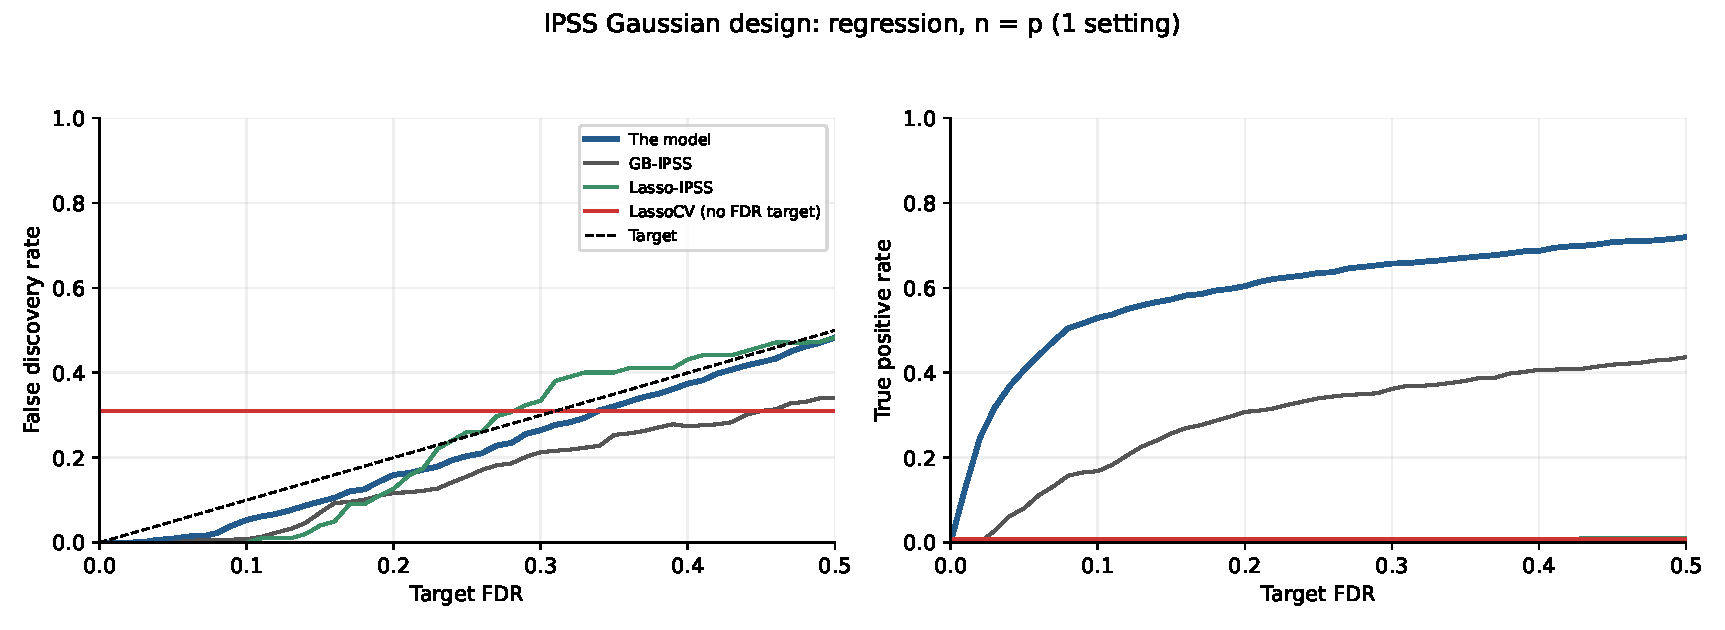
\includegraphics[page=1,width=\linewidth]{final_model_note_figures.pdf}
\caption{Small-sample adaptation of the IPSS Gaussian design.}
\label{fig:assessment-1}
\end{figure}

\begin{figure}[H]
\textbf{Gaussian regression, $n=\max\{50,\lfloor0.8p\rfloor\}$.} These 100 datasets use $p=\operatorname{round}(\exp U)$, $U\sim\mathrm{Uniform}(\log50,\log500)$ and $n=\max\{50,\lfloor0.8p\rfloor\}$. Draw Gaussian predictors with covariance $\Sigma_{jk}=0.5^{|j-k|}$ and standardize their columns. Choose $k$ uniformly from $\{5,\ldots,15\}$ and choose $k$ relevant columns uniformly. The uncentered signal is $\sum_{j\in S}\exp(-X_{ij}^2)$. Center the signal, draw SNR uniformly from $[0.5,2]$, and add independent Gaussian noise with variance equal to the signal variance divided by SNR. Finally center the response.
\par\medskip\centering
\includegraphics[page=2,width=\linewidth]{final_model_note_figures.pdf}
\caption{Small-sample adaptation of the IPSS Gaussian design.}
\label{fig:assessment-2}
\end{figure}

\begin{figure}[H]
\textbf{Gaussian classification, $n=p$.} These 100 datasets use $p=\operatorname{round}(\exp U)$, $U\sim\mathrm{Uniform}(\log50,\log500)$ and $n=p$. Draw Gaussian predictors with covariance $\Sigma_{jk}=0.5^{|j-k|}$ and standardize their columns. Choose $k$ uniformly from $\{5,\ldots,15\}$ and choose $k$ relevant columns uniformly. The uncentered signal is $\sum_{j\in S}\exp(-X_{ij}^2)$. Center the signal, draw $u\sim\mathrm{Uniform}(1,3)$, and generate independent Bernoulli responses with probabilities $\operatorname{sigmoid}(u s_i)$.
\par\medskip\centering
\includegraphics[page=3,width=\linewidth]{final_model_note_figures.pdf}
\caption{Small-sample adaptation of the IPSS Gaussian design.}
\label{fig:assessment-3}
\end{figure}

\begin{figure}[H]
\textbf{Gaussian classification, $n=\max\{50,\lfloor0.8p\rfloor\}$.} These 100 datasets use $p=\operatorname{round}(\exp U)$, $U\sim\mathrm{Uniform}(\log50,\log500)$ and $n=\max\{50,\lfloor0.8p\rfloor\}$. Draw Gaussian predictors with covariance $\Sigma_{jk}=0.5^{|j-k|}$ and standardize their columns. Choose $k$ uniformly from $\{5,\ldots,15\}$ and choose $k$ relevant columns uniformly. The uncentered signal is $\sum_{j\in S}\exp(-X_{ij}^2)$. Center the signal, draw $u\sim\mathrm{Uniform}(1,3)$, and generate independent Bernoulli responses with probabilities $\operatorname{sigmoid}(u s_i)$.
\par\medskip\centering
\includegraphics[page=4,width=\linewidth]{final_model_note_figures.pdf}
\caption{Small-sample adaptation of the IPSS Gaussian design.}
\label{fig:assessment-4}
\end{figure}

\subsection{RNA-seq design adapted from IPSS}
The source is the ovarian RNA-seq matrix released with the paper:
569 patients and 6,426 measured genes. Sample $n$ rows without replacement,
exclude columns constant in those rows, and sample $p$ remaining columns
without replacement. Standardize each selected column to mean zero and
variance one. Draw $k$ uniformly from $\{10,\ldots,30\}$ and choose $k$
relevant columns uniformly without replacement.

Draw the number of groups $G$ uniformly from $\lfloor k/2\rfloor$ through
$k$. Randomly permute the $k$ relevant columns and uniformly choose $G-1$
cut positions among the $k-1$ internal positions, giving $G$ nonempty groups.
For each group $S_g$, sum its columns and standardize the sum across samples
to obtain $z_g$. Independently draw a function for each group:
\[
 f(z)=\begin{cases}
 d_1[1+\tanh(a(d_2z-b))]/2,&\text{with probability }1/2,\\
 d_1\exp(-c z^2),&\text{with probability }1/2,
 \end{cases}
\]
where $a\sim U(0.5,1.5)$, $b\sim U(-1,1)$, $c\sim U(1,3)$ and
$d_1,d_2$ are independent equiprobable signs. The parameters and the choice
between the two functions are drawn once per group and shared across its
samples. Sum the group contributions and center the signal:
\[
 r_i=\sum_{g=1}^G f_g(z_{ig}),\qquad
 s_i=r_i-\frac1n\sum_{\ell=1}^n r_\ell.
\]
Generate responses from $s$ using the same rules as in the Gaussian design:
for regression, draw one SNR from $U(0.5,2)$, add independent Gaussian noise
with variance $(n^{-1}\sum_i s_i^2)/\mathrm{SNR}$, and center the response;
for classification, draw one $u\sim U(1,3)$ and independently sample
$y_i\sim\mathrm{Bernoulli}([1+\exp(-u s_i)]^{-1})$ conditional on the
predictor matrix, the generated signal functions and $u$.

\begin{figure}[H]
\textbf{RNA-seq regression, $n=p$.} These 100 datasets use $p=\operatorname{round}(\exp U)$, $U\sim\mathrm{Uniform}(\log50,\log500)$ and $n=p$. Sample rows and varying columns without replacement from the $569\times6426$ ovarian RNA-seq matrix, then standardize each selected column. Choose $k\in\{10,\ldots,30\}$ relevant genes uniformly and split them into $G\in\{\lfloor k/2\rfloor,\ldots,k\}$ random nonempty groups. Standardize each group sum, apply an independently randomized tanh or Gaussian-bump function as specified above, sum the outputs, and center the result $s$. Draw SNR uniformly from $[0.5,2]$ and add independent Gaussian noise with variance $\operatorname{var}(s)/\mathrm{SNR}$. Finally center the response.
\par\medskip\centering
\includegraphics[page=5,width=\linewidth]{final_model_note_figures.pdf}
\caption{Small-sample adaptation of the IPSS RNA-seq design.}
\label{fig:assessment-5}
\end{figure}

\begin{figure}[H]
\textbf{RNA-seq regression, $n=\max\{50,\lfloor0.8p\rfloor\}$.} These 100 datasets use $p=\operatorname{round}(\exp U)$, $U\sim\mathrm{Uniform}(\log50,\log500)$ and $n=\max\{50,\lfloor0.8p\rfloor\}$. Sample rows and varying columns without replacement from the $569\times6426$ ovarian RNA-seq matrix, then standardize each selected column. Choose $k\in\{10,\ldots,30\}$ relevant genes uniformly and split them into $G\in\{\lfloor k/2\rfloor,\ldots,k\}$ random nonempty groups. Standardize each group sum, apply an independently randomized tanh or Gaussian-bump function as specified above, sum the outputs, and center the result $s$. Draw SNR uniformly from $[0.5,2]$ and add independent Gaussian noise with variance $\operatorname{var}(s)/\mathrm{SNR}$. Finally center the response.
\par\medskip\centering
\includegraphics[page=6,width=\linewidth]{final_model_note_figures.pdf}
\caption{Small-sample adaptation of the IPSS RNA-seq design.}
\label{fig:assessment-6}
\end{figure}

\begin{figure}[H]
\textbf{RNA-seq classification, $n=p$.} These 100 datasets use $p=\operatorname{round}(\exp U)$, $U\sim\mathrm{Uniform}(\log50,\log500)$ and $n=p$. Sample rows and varying columns without replacement from the $569\times6426$ ovarian RNA-seq matrix, then standardize each selected column. Choose $k\in\{10,\ldots,30\}$ relevant genes uniformly and split them into $G\in\{\lfloor k/2\rfloor,\ldots,k\}$ random nonempty groups. Standardize each group sum, apply an independently randomized tanh or Gaussian-bump function as specified above, sum the outputs, and center the result $s$. Draw $u\sim\mathrm{Uniform}(1,3)$ and sample independent $y_i\sim\mathrm{Bernoulli}(\operatorname{sigmoid}(u s_i))$.
\par\medskip\centering
\includegraphics[page=7,width=\linewidth]{final_model_note_figures.pdf}
\caption{Small-sample adaptation of the IPSS RNA-seq design.}
\label{fig:assessment-7}
\end{figure}

\begin{figure}[H]
\textbf{RNA-seq classification, $n=\max\{50,\lfloor0.8p\rfloor\}$.} These 100 datasets use $p=\operatorname{round}(\exp U)$, $U\sim\mathrm{Uniform}(\log50,\log500)$ and $n=\max\{50,\lfloor0.8p\rfloor\}$. Sample rows and varying columns without replacement from the $569\times6426$ ovarian RNA-seq matrix, then standardize each selected column. Choose $k\in\{10,\ldots,30\}$ relevant genes uniformly and split them into $G\in\{\lfloor k/2\rfloor,\ldots,k\}$ random nonempty groups. Standardize each group sum, apply an independently randomized tanh or Gaussian-bump function as specified above, sum the outputs, and center the result $s$. Draw $u\sim\mathrm{Uniform}(1,3)$ and sample independent $y_i\sim\mathrm{Bernoulli}(\operatorname{sigmoid}(u s_i))$.
\par\medskip\centering
\includegraphics[page=8,width=\linewidth]{final_model_note_figures.pdf}
\caption{Small-sample adaptation of the IPSS RNA-seq design.}
\label{fig:assessment-8}
\end{figure}

\subsection{Results on the additional benchmarks}
The two additional synthetic designs and the MNIST and BASEHOCK
semi-simulations contribute 1,200 datasets across 12 settings. Each of the
six figures averages 100 draws with $n=p$ and 100 draws with
$n=\max\{50,\lfloor0.8p\rfloor\}$. The following numerical comparisons
use target FDR $\alpha=0.10$; the appendix shows the full target range
from 0 to 0.50 for every method and setting.


\textbf{Synthetic benchmarks.} In the sparse linear design (Figure~\ref{fig:assessment-13}), the model achieves 74.1\% TPR and 11.7\% FDR, compared with 45.8\% TPR and 6.8\% FDR for GB-IPSS and 60.7\% TPR and 6.6\% FDR for Lasso-IPSS. The higher TPR comes with empirical FDR above the 10\% target. In Friedman \#1 (Figure~\ref{fig:assessment-14}), the model achieves 78.9\% TPR and 2.2\% FDR, whereas GB-IPSS achieves 91.0\% TPR and 4.7\% FDR and Lasso-IPSS achieves 77.0\% TPR and 7.4\% FDR. GB-IPSS therefore finds more true variables in this design while also remaining below the stated FDR target.

\textbf{Real predictors with linear responses.} On MNIST (Figure~\ref{fig:assessment-21}), the model achieves 34.7\% TPR and 6.2\% FDR, compared with 41.4\% TPR and 28.4\% FDR for GB-IPSS and 12.0\% TPR and 2.5\% FDR for Lasso-IPSS. On BASEHOCK (Figure~\ref{fig:assessment-23}), the corresponding results are 32.3\% TPR and 6.1\% FDR for the model, 28.4\% TPR and 38.3\% FDR for GB-IPSS, and 7.3\% TPR and 0.5\% FDR. In both designs, the model finds more true variables than Lasso-IPSS and has lower empirical FDR than GB-IPSS.

\textbf{Real predictors with square responses.} On MNIST (Figure~\ref{fig:assessment-22}), the model achieves 9.5\% TPR and 4.0\% FDR, compared with 7.1\% TPR and 11.5\% FDR for GB-IPSS and 1.1\% TPR and 0.4\% FDR for Lasso-IPSS. On BASEHOCK (Figure~\ref{fig:assessment-24}), the model achieves 9.4\% TPR and 3.9\% FDR, compared with 12.1\% TPR and 28.5\% FDR for GB-IPSS and 0.0\% TPR and 0.0\% FDR for Lasso-IPSS. The model selects fewer than one in ten true variables in both square-response designs at $\alpha=0.10$, so substantial power limitations remain.

\textbf{LassoCV.} Across these six comparisons, LassoCV has TPR between 47.6\% and 97.8\%, with FDR between 63.6\% and 73.6\%. Its large selected sets recover many true variables but also include many false selections; LassoCV has no target-FDR input.

% BEGIN LOCAL FDR COMPARISON

\subsection{Comparison with local false-discovery methods}
The following comparison reuses all 4,000 datasets above, including the
same predictor matrices, responses and planted relevant columns.
The model's saved selections are reused without refitting or changing its
thresholds. The additional methods receive only $X$ and $y$.
Their implementation choices were fixed before computing their test results.

\textbf{Sun--Cai.} For each column, calculate the correlation with $y$,
convert it to a $t$ statistic with $n-2$ degrees of freedom, and transform
its null cumulative probability to a standard normal score $z_j$.
For binary responses this is also the pooled two-sample $t$ test on that
column across the two response groups. Estimate
$\ell_j=\widehat\pi_0\phi(z_j)/\widehat f(z_j)$, truncated to $[0,1]$,
using the theoretical $N(0,1)$ null. The null proportion uses the
Jin--Cai estimator \cite{jincai}; the density uses a Gaussian kernel with
bandwidth chosen by unbiased cross-validation. Implement the Sun--Cai
selection rule \cite{suncai}: sort these scores and take the largest
complete-tie prefix whose average is at most $\alpha$.
This is an implementation of the published rule with the numerical choices
recorded in \code{data/lfdr_comparison_protocol.json}.

\textbf{Cumulative $\ell$-value.} Use the same $z_j$ values, but replace
the estimated density by the mixture in Abraham, Castillo and Roquain
\cite{cumulativeell}. Its null density is standard normal, and its
alternative density is
$g(z)=(1-e^{-z^2/2})/(\sqrt{2\pi}z^2)$, with its continuous value at zero.
Estimate the nonnull mixture weight by maximum likelihood over $[1/p,1]$.
Calculate each variable's posterior null probability and apply the same
cumulative-average rule. The paper studies independent Gaussian
coordinates; using regression-derived $z$ scores here is an application
to the present datasets, not a reproduction of that paper's simulation.

\textbf{Lasso local FDR.} Use the authors' \code{ncvreg} implementation
of Miller and Breheny \cite{millerbreheny}. Fit a Lasso with ten-fold
cross-validation and use the penalty with minimum validation error.
The response family is Gaussian for regression and binomial for
classification. Compute \code{local_mfdr(method="ashr")} for all columns.
The \emph{pointwise} curve selects columns with local FDR at most $\alpha$,
as in the paper's simulation. The \emph{cumulative} curve instead applies
the cumulative-average rule to those same scores. The latter is explicitly
an additional version of the selection rule. Package defaults are retained
otherwise; software versions and random seeds accompany the results.

\textbf{What is being compared.} Every method is scored against the
same columns that directly generated $y$. A correlated but unplanted
column therefore counts as a false selection. This differs from the
marginal-association null used by these literature methods.
Nonlinear responses can also contain relevant columns with zero marginal
linear association. The comparison measures their usefulness for the
present variable-selection task; their original FDR guarantees do not
automatically apply to these correlated, nonlinear datasets.

\textbf{Results.} Table~\ref{tab:lfdr-comparison} reports both error rate
and power at target $\alpha=0.10$, averaged equally across the 40 settings.
Standard errors reflect independent replicates within each fixed setting.
The paired curves cover all targets from 0 to 0.50; the appendix includes
every setting, ordered by simulated predictors and then real predictors.
No setting was removed based on its results.
\begin{table}[H]
\centering\small
\begin{tabular}{lrrrr}
\toprule
Method & TPR & TPR SE & FDR & FDR SE\\
\midrule
The model & 28.9\% & 0.4\% & 4.9\% & 0.2\%\\
Sun--Cai & 54.3\% & 0.3\% & 54.4\% & 0.4\%\\
Cumulative $\ell$-value & 48.6\% & 0.4\% & 44.4\% & 0.4\%\\
Lasso local FDR: pointwise & 31.3\% & 0.3\% & 19.1\% & 0.4\%\\
Lasso local FDR: cumulative & 34.8\% & 0.3\% & 22.4\% & 0.4\%\\
\bottomrule
\end{tabular}
\caption{All 4,000 existing datasets, target FDR $0.10$. All entries are percentages; SE denotes standard error.}
\label{tab:lfdr-comparison}
\end{table}
The model has 28.9\% TPR and 4.9\% FDR at this target. Relative to Sun--Cai, its TPR difference is -25.5 percentage points (paired 95\% normal interval -26.2 to -24.7). Relative to Cumulative $\ell$-value, its TPR difference is -19.7 percentage points (paired 95\% normal interval -20.6 to -18.8). Relative to Lasso local FDR: pointwise, its TPR difference is -2.4 percentage points (paired 95\% normal interval -3.1 to -1.7). Relative to Lasso local FDR: cumulative, its TPR difference is -5.9 percentage points (paired 95\% normal interval -6.6 to -5.2). These power differences must be interpreted together with the measured FDRs in the table.

At this target, the model is the only displayed method with overall empirical FDR below 10\%. Its empirical FDR exceeds 10\% in 4 of the 40 individual settings; the corresponding counts are 34 for Sun--Cai, 28 for Cumulative $\ell$-value, 22 for Lasso local FDR: pointwise, 27 for Lasso local FDR: cumulative. An acceptable overall average therefore does not establish control in every setting.

For the 1,600 datasets with simulated predictors, the model achieves 51.9\% TPR and 6.3\% FDR, compared with 38.3\% TPR and 6.6\% FDR for the cumulative Lasso rule. For the 2,400 datasets with real predictors, the model achieves 13.6\% TPR and 4.0\% FDR, compared with 32.5\% TPR and 32.8\% FDR for that rule. On real predictors, several alternatives recover more planted variables while also selecting many correlated, unplanted columns. The complete figures expose this tradeoff rather than ranking methods by TPR alone.

\begin{figure}[H]
\textbf{All existing assessment settings.} These 4,000 datasets comprise 40 fixed settings with 100 independent draws each: 1,600 datasets use simulated predictors and 2,400 use real predictors with simulated responses. Each draw satisfies $50\le n\le p\le500$. The same matrices, responses, planted supports and sample-size regimes are used for all methods. The preceding sections specify each generator; all settings receive equal weight.
\par\medskip\centering
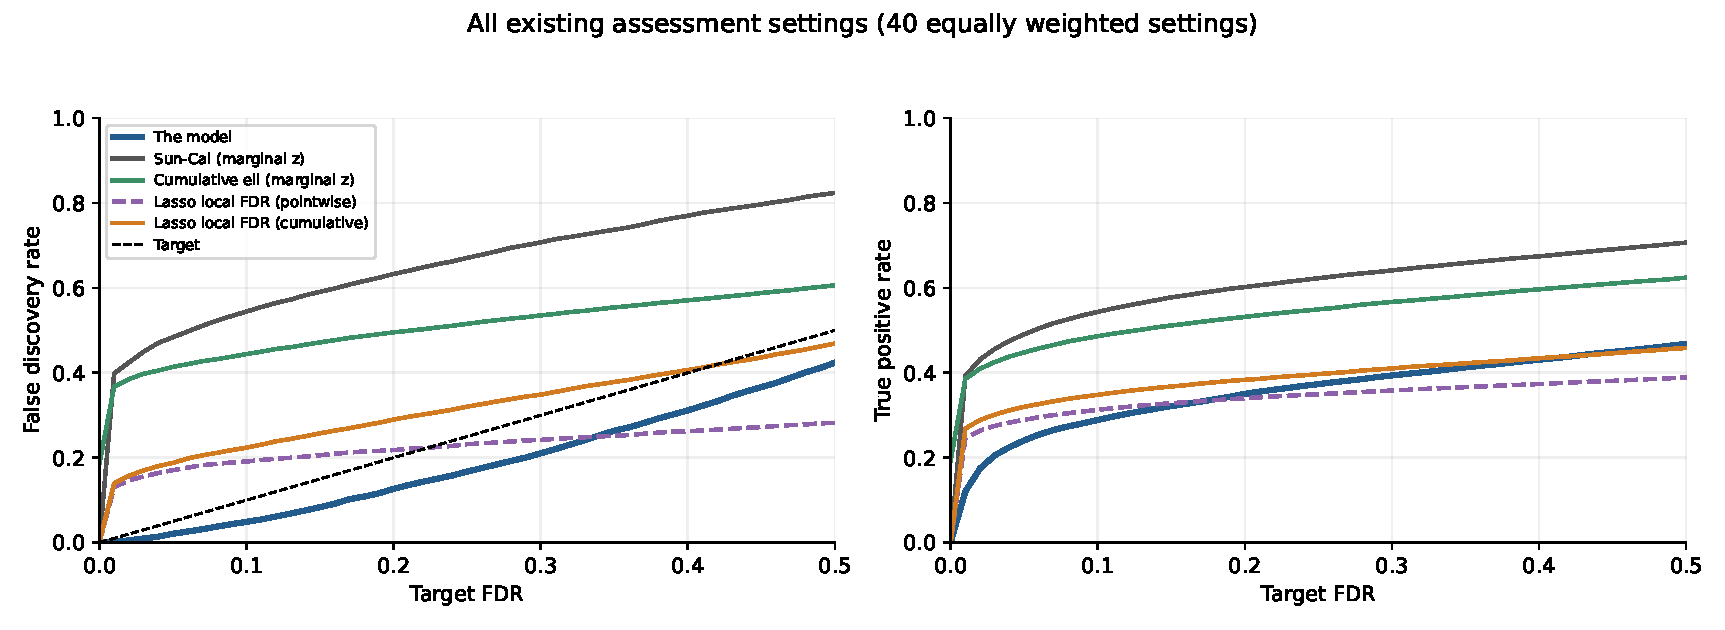
\includegraphics[page=1,width=\linewidth]{lfdr_comparison_figures.pdf}
\caption{The model and local-FDR methods on all existing assessment settings.}
\label{fig:lfdr-overall}
\end{figure}
% END LOCAL FDR COMPARISON

\begingroup\small
\begin{thebibliography}{99}
\bibitem{ipss} O.~Melikechi and J.~W.~Miller.
\emph{Integrated path stability selection}. arXiv:2403.15877, 2025.
\bibitem{ipssgb} O.~Melikechi, D.~B.~Dunson, and J.~W.~Miller.
\emph{Nonparametric IPSS: Fast, flexible feature selection with false discovery control}.
Bioinformatics, 2025. doi:10.1093/bioinformatics/btaf299.
The specification also uses the supplement in arXiv:2410.02208v3.
Code and RNA-seq data: \url{https://github.com/omelikechi/ipss_bioinformatics}.
\bibitem{xgboost} T.~Chen and C.~Guestrin.
\emph{XGBoost: A Scalable Tree Boosting System}. KDD, 2016, pp.~785--794.
\bibitem{scikitfeature} J.~Li et al. scikit-feature dataset collection.
ISOLET subset, COIL20 and BASEHOCK matrices, repository snapshot
\code{48cffad4e88ff4b9d2f1c7baffb314d1b3303792}.
\url{https://jundongl.github.io/scikit-feature/datasets}.
\bibitem{har} D.~Anguita et al. Human Activity Recognition Using Smartphones.
UCI Machine Learning Repository. doi:10.24432/C54S4K.
\bibitem{knockoffexample} M.~Sesia. \emph{Controlled variable Selection with Model-X Knockoffs}.
Authors' software example, 2017.
\url{https://web.stanford.edu/group/candes/knockoffs/software/knockoffs/r/knockoff.html}.
\bibitem{friedman1} J.~H.~Friedman. \emph{Multivariate adaptive regression splines}.
Annals of Statistics, 19(1):1--67, 1991. Generator specification:
\url{https://scikit-learn.org/stable/modules/generated/sklearn.datasets.make_friedman1.html}.
\bibitem{mnist} TensorFlow/Keras. MNIST handwritten-digit dataset.
Official training split: 60,000 images, each $28\times28$ pixels.
\url{https://www.tensorflow.org/api_docs/python/tf/keras/datasets/mnist/load_data}.
% BEGIN LOCAL FDR COMPARISON

\bibitem{suncai} W.~Sun and T.~T.~Cai. Oracle and adaptive compound decision rules for false discovery rate control.
Journal of the American Statistical Association, 102:901--912, 2007. doi:10.1198/016214507000000545.
\bibitem{jincai} J.~Jin and T.~T.~Cai. Estimating the null and the proportion of nonnull effects in large-scale multiple comparisons.
Journal of the American Statistical Association, 102:495--506, 2007. doi:10.1198/016214507000000167.
\bibitem{cumulativeell} K.~Abraham, I.~Castillo, and E.~Roquain. Empirical Bayes cumulative $\ell$-value multiple testing procedure for sparse sequences.
arXiv:2102.00929v3, 2022.
\bibitem{millerbreheny} R.~Miller and P.~Breheny. Feature-specific inference for penalized regression using local false discovery rates.
Statistics in Medicine, 42:1412--1429, 2023. doi:10.1002/sim.9678.
% END LOCAL FDR COMPARISON
\end{thebibliography}
\endgroup
\newpage\appendix\section{Additional Small-Sample Evaluations}
\subsection{Simulated test datasets}

\begin{figure}[H]
\textbf{Simple linear response.} These 200 datasets give equal weight to 100 draws with $n=p$ and 100 with $n=\max\{50,\lfloor0.8p\rfloor\}$; in both, $p=\operatorname{round}(\exp U)$, $U\sim\mathrm{Uniform}(\log50,\log500)$. Generate Gaussian predictors with $\Sigma_{jk}=0.5^{|j-k|}$ and standardize their columns. Choose six relevant columns uniformly. Form the signal $v_i=\sum_{j\in S}X_{ij}$, center it and scale it to standard deviation one, and set $y_i=v_i+\varepsilon_i$ with independent $\varepsilon_i\sim N(0,1)$. Thus SNR is 1. Finally center the response. All draws are retained.
\par\medskip\centering
\includegraphics[page=9,width=\linewidth]{final_model_note_figures.pdf}
\caption{Prespecified supplemental setting; both sample-size regimes receive equal weight.}
\label{fig:assessment-9}
\end{figure}

\begin{figure}[H]
\textbf{Simple square response.} These 200 datasets give equal weight to 100 draws with $n=p$ and 100 with $n=\max\{50,\lfloor0.8p\rfloor\}$; in both, $p=\operatorname{round}(\exp U)$, $U\sim\mathrm{Uniform}(\log50,\log500)$. Generate Gaussian predictors with $\Sigma_{jk}=0.5^{|j-k|}$ and standardize their columns. Choose six relevant columns uniformly. Form the signal $v_i=\sum_{j\in S}X_{ij}^2$, center it and scale it to standard deviation one, and set $y_i=v_i+\varepsilon_i$ with independent $\varepsilon_i\sim N(0,1)$. Thus SNR is 1. Finally center the response. All draws are retained.
\par\medskip\centering
\includegraphics[page=10,width=\linewidth]{final_model_note_figures.pdf}
\caption{Prespecified supplemental setting; both sample-size regimes receive equal weight.}
\label{fig:assessment-10}
\end{figure}

\begin{figure}[H]
\textbf{Simple sine response.} These 200 datasets give equal weight to 100 draws with $n=p$ and 100 with $n=\max\{50,\lfloor0.8p\rfloor\}$; in both, $p=\operatorname{round}(\exp U)$, $U\sim\mathrm{Uniform}(\log50,\log500)$. Generate Gaussian predictors with $\Sigma_{jk}=0.5^{|j-k|}$ and standardize their columns. Choose six relevant columns uniformly. Form the signal $v_i=\sum_{j\in S}\sin(X_{ij})$, center it and scale it to standard deviation one, and set $y_i=v_i+\varepsilon_i$ with independent $\varepsilon_i\sim N(0,1)$. Thus SNR is 1. Finally center the response. All draws are retained.
\par\medskip\centering
\includegraphics[page=11,width=\linewidth]{final_model_note_figures.pdf}
\caption{Prespecified supplemental setting; both sample-size regimes receive equal weight.}
\label{fig:assessment-11}
\end{figure}

\begin{figure}[H]
\textbf{Simple interaction response.} These 200 datasets give equal weight to 100 draws with $n=p$ and 100 with $n=\max\{50,\lfloor0.8p\rfloor\}$; in both, $p=\operatorname{round}(\exp U)$, $U\sim\mathrm{Uniform}(\log50,\log500)$. Generate Gaussian predictors with $\Sigma_{jk}=0.5^{|j-k|}$ and standardize their columns. Choose six relevant columns uniformly. Form the signal $v_i=X_{i,j_1}X_{i,j_2}+X_{i,j_3}X_{i,j_4}+X_{i,j_5}X_{i,j_6}$, center it and scale it to standard deviation one, and set $y_i=v_i+\varepsilon_i$ with independent $\varepsilon_i\sim N(0,1)$. Thus SNR is 1. Finally center the response. All draws are retained.
\par\medskip\centering
\includegraphics[page=12,width=\linewidth]{final_model_note_figures.pdf}
\caption{Prespecified supplemental setting; both sample-size regimes receive equal weight.}
\label{fig:assessment-12}
\end{figure}

\begin{figure}[H]
\textbf{Sparse linear response with correlated Gaussian predictors.} These 200 datasets give equal weight to 100 draws with $n=p$ and 100 with $n=\max\{50,\lfloor0.8p\rfloor\}$; in both, $p=\operatorname{round}(\exp U)$, $U\sim\mathrm{Uniform}(\log50,\log500)$. Draw independent rows $X_i\sim N(0,\Sigma)$ with $\Sigma_{jk}=0.25^{|j-k|}$. Choose ten relevant columns uniformly and set $y_i=(4.5/\sqrt n)\sum_{j\in S}X_{ij}+\varepsilon_i$, with independent $\varepsilon_i\sim N(0,1)$. This is the sparse linear benchmark family used in the model-X knockoffs authors\textquotesingle{} example \cite{knockoffexample}. We retain its correlation, coefficient scale and noise variance, but use ten relevant columns instead of sixty to accommodate $p\ge50$, and replace its fixed dimensions by the rule above. The generator does not sample-standardize $X$ or center $y$. All draws are retained.
\par\medskip\centering
\includegraphics[page=13,width=\linewidth]{final_model_note_figures.pdf}
\caption{Prespecified supplemental setting; both sample-size regimes receive equal weight.}
\label{fig:assessment-13}
\end{figure}

\begin{figure}[H]
\textbf{Friedman \#1 nonlinear regression.} These 200 datasets give equal weight to 100 draws with $n=p$ and 100 with $n=\max\{50,\lfloor0.8p\rfloor\}$; in both, $p=\operatorname{round}(\exp U)$, $U\sim\mathrm{Uniform}(\log50,\log500)$. Draw all entries of $X$ independently from $U(0,1)$. Before permuting columns, set $y_i=10\sin(\pi X_{i1}X_{i2})+20(X_{i3}-0.5)^2+10X_{i4}+5X_{i5}+\varepsilon_i$, with independent $\varepsilon_i\sim N(0,1)$. Only these five columns are relevant. Use the standard Friedman \#1 generator \cite{friedman1}, then randomly permute all columns and track the five relevant indices. The generator does not standardize $X$ or center $y$. All draws are retained.
\par\medskip\centering
\includegraphics[page=14,width=\linewidth]{final_model_note_figures.pdf}
\caption{Prespecified supplemental setting; both sample-size regimes receive equal weight.}
\label{fig:assessment-14}
\end{figure}
\subsection{Real predictors with simulated responses}

\begin{figure}[H]
\textbf{ISOLET predictors with a linear response.} These 200 datasets give equal weight to 100 draws with $n=p$ and 100 with $n=\max\{50,\lfloor0.8p\rfloor\}$; in both, $p=\operatorname{round}(\exp U)$, $U\sim\mathrm{Uniform}(\log50,\log500)$. The fixed real predictor pool has 1,560 rows and 617 columns. The pool is the scikit-feature subset of spoken-letter acoustic measurements \cite{scikitfeature}. Sample rows without replacement, remove columns constant in those rows, sample $p$ remaining columns without replacement, and standardize them. Original response labels are unused. Choose six relevant columns uniformly. Form the signal $v_i=\sum_{j\in S}X_{ij}$, center it and scale it to standard deviation one, and set $y_i=v_i+\varepsilon_i$ with independent $\varepsilon_i\sim N(0,1)$. Thus SNR is 1. Finally center the response. All draws are retained.
\par\medskip\centering
\includegraphics[page=15,width=\linewidth]{final_model_note_figures.pdf}
\caption{Prespecified supplemental setting; both sample-size regimes receive equal weight.}
\label{fig:assessment-15}
\end{figure}

\begin{figure}[H]
\textbf{ISOLET predictors with a square response.} These 200 datasets give equal weight to 100 draws with $n=p$ and 100 with $n=\max\{50,\lfloor0.8p\rfloor\}$; in both, $p=\operatorname{round}(\exp U)$, $U\sim\mathrm{Uniform}(\log50,\log500)$. The fixed real predictor pool has 1,560 rows and 617 columns. The pool is the scikit-feature subset of spoken-letter acoustic measurements \cite{scikitfeature}. Sample rows without replacement, remove columns constant in those rows, sample $p$ remaining columns without replacement, and standardize them. Original response labels are unused. Choose six relevant columns uniformly. Form the signal $v_i=\sum_{j\in S}X_{ij}^2$, center it and scale it to standard deviation one, and set $y_i=v_i+\varepsilon_i$ with independent $\varepsilon_i\sim N(0,1)$. Thus SNR is 1. Finally center the response. All draws are retained.
\par\medskip\centering
\includegraphics[page=16,width=\linewidth]{final_model_note_figures.pdf}
\caption{Prespecified supplemental setting; both sample-size regimes receive equal weight.}
\label{fig:assessment-16}
\end{figure}

\begin{figure}[H]
\textbf{HAR predictors with a linear response.} These 200 datasets give equal weight to 100 draws with $n=p$ and 100 with $n=\max\{50,\lfloor0.8p\rfloor\}$; in both, $p=\operatorname{round}(\exp U)$, $U\sim\mathrm{Uniform}(\log50,\log500)$. The fixed real predictor pool has 10,299 rows and 561 columns. The pool combines the original UCI train and test predictor files of smartphone sensor summaries \cite{har}. Sample rows without replacement, remove columns constant in those rows, sample $p$ remaining columns without replacement, and standardize them. Original response labels are unused. Choose six relevant columns uniformly. Form the signal $v_i=\sum_{j\in S}X_{ij}$, center it and scale it to standard deviation one, and set $y_i=v_i+\varepsilon_i$ with independent $\varepsilon_i\sim N(0,1)$. Thus SNR is 1. Finally center the response. All draws are retained.
\par\medskip\centering
\includegraphics[page=17,width=\linewidth]{final_model_note_figures.pdf}
\caption{Prespecified supplemental setting; both sample-size regimes receive equal weight.}
\label{fig:assessment-17}
\end{figure}

\begin{figure}[H]
\textbf{HAR predictors with a square response.} These 200 datasets give equal weight to 100 draws with $n=p$ and 100 with $n=\max\{50,\lfloor0.8p\rfloor\}$; in both, $p=\operatorname{round}(\exp U)$, $U\sim\mathrm{Uniform}(\log50,\log500)$. The fixed real predictor pool has 10,299 rows and 561 columns. The pool combines the original UCI train and test predictor files of smartphone sensor summaries \cite{har}. Sample rows without replacement, remove columns constant in those rows, sample $p$ remaining columns without replacement, and standardize them. Original response labels are unused. Choose six relevant columns uniformly. Form the signal $v_i=\sum_{j\in S}X_{ij}^2$, center it and scale it to standard deviation one, and set $y_i=v_i+\varepsilon_i$ with independent $\varepsilon_i\sim N(0,1)$. Thus SNR is 1. Finally center the response. All draws are retained.
\par\medskip\centering
\includegraphics[page=18,width=\linewidth]{final_model_note_figures.pdf}
\caption{Prespecified supplemental setting; both sample-size regimes receive equal weight.}
\label{fig:assessment-18}
\end{figure}

\begin{figure}[H]
\textbf{COIL20 predictors with a linear response.} These 200 datasets give equal weight to 100 draws with $n=p$ and 100 with $n=\max\{50,\lfloor0.8p\rfloor\}$; in both, $p=\operatorname{round}(\exp U)$, $U\sim\mathrm{Uniform}(\log50,\log500)$. The fixed real predictor pool has 1,440 rows and 1,024 columns. The pool contains flattened object images from COIL20, distributed by scikit-feature \cite{scikitfeature}. Sample rows without replacement, remove columns constant in those rows, sample $p$ remaining columns without replacement, and standardize them. Original response labels are unused. Choose six relevant columns uniformly. Form the signal $v_i=\sum_{j\in S}X_{ij}$, center it and scale it to standard deviation one, and set $y_i=v_i+\varepsilon_i$ with independent $\varepsilon_i\sim N(0,1)$. Thus SNR is 1. Finally center the response. All draws are retained.
\par\medskip\centering
\includegraphics[page=19,width=\linewidth]{final_model_note_figures.pdf}
\caption{Prespecified supplemental setting; both sample-size regimes receive equal weight.}
\label{fig:assessment-19}
\end{figure}

\begin{figure}[H]
\textbf{COIL20 predictors with a square response.} These 200 datasets give equal weight to 100 draws with $n=p$ and 100 with $n=\max\{50,\lfloor0.8p\rfloor\}$; in both, $p=\operatorname{round}(\exp U)$, $U\sim\mathrm{Uniform}(\log50,\log500)$. The fixed real predictor pool has 1,440 rows and 1,024 columns. The pool contains flattened object images from COIL20, distributed by scikit-feature \cite{scikitfeature}. Sample rows without replacement, remove columns constant in those rows, sample $p$ remaining columns without replacement, and standardize them. Original response labels are unused. Choose six relevant columns uniformly. Form the signal $v_i=\sum_{j\in S}X_{ij}^2$, center it and scale it to standard deviation one, and set $y_i=v_i+\varepsilon_i$ with independent $\varepsilon_i\sim N(0,1)$. Thus SNR is 1. Finally center the response. All draws are retained.
\par\medskip\centering
\includegraphics[page=20,width=\linewidth]{final_model_note_figures.pdf}
\caption{Prespecified supplemental setting; both sample-size regimes receive equal weight.}
\label{fig:assessment-20}
\end{figure}

\begin{figure}[H]
\textbf{MNIST predictors with a linear response.} These 200 datasets give equal weight to 100 draws with $n=p$ and 100 with $n=\max\{50,\lfloor0.8p\rfloor\}$; in both, $p=\operatorname{round}(\exp U)$, $U\sim\mathrm{Uniform}(\log50,\log500)$. The fixed real predictor pool has 60,000 rows and 784 columns. The pool is the official MNIST training set, with each $28\times28$ grayscale image flattened to 784 pixel measurements \cite{mnist}. Sample rows without replacement, remove columns constant in those rows, sample $p$ remaining columns without replacement, and standardize them. Original response labels are unused. Choose six relevant columns uniformly. Form the signal $v_i=\sum_{j\in S}X_{ij}$, center it and scale it to standard deviation one, and set $y_i=v_i+\varepsilon_i$ with independent $\varepsilon_i\sim N(0,1)$. Thus SNR is 1. Finally center the response. All draws are retained.
\par\medskip\centering
\includegraphics[page=21,width=\linewidth]{final_model_note_figures.pdf}
\caption{Prespecified supplemental setting; both sample-size regimes receive equal weight.}
\label{fig:assessment-21}
\end{figure}

\begin{figure}[H]
\textbf{MNIST predictors with a square response.} These 200 datasets give equal weight to 100 draws with $n=p$ and 100 with $n=\max\{50,\lfloor0.8p\rfloor\}$; in both, $p=\operatorname{round}(\exp U)$, $U\sim\mathrm{Uniform}(\log50,\log500)$. The fixed real predictor pool has 60,000 rows and 784 columns. The pool is the official MNIST training set, with each $28\times28$ grayscale image flattened to 784 pixel measurements \cite{mnist}. Sample rows without replacement, remove columns constant in those rows, sample $p$ remaining columns without replacement, and standardize them. Original response labels are unused. Choose six relevant columns uniformly. Form the signal $v_i=\sum_{j\in S}X_{ij}^2$, center it and scale it to standard deviation one, and set $y_i=v_i+\varepsilon_i$ with independent $\varepsilon_i\sim N(0,1)$. Thus SNR is 1. Finally center the response. All draws are retained.
\par\medskip\centering
\includegraphics[page=22,width=\linewidth]{final_model_note_figures.pdf}
\caption{Prespecified supplemental setting; both sample-size regimes receive equal weight.}
\label{fig:assessment-22}
\end{figure}

\begin{figure}[H]
\textbf{BASEHOCK predictors with a linear response.} These 200 datasets give equal weight to 100 draws with $n=p$ and 100 with $n=\max\{50,\lfloor0.8p\rfloor\}$; in both, $p=\operatorname{round}(\exp U)$, $U\sim\mathrm{Uniform}(\log50,\log500)$. The fixed real predictor pool has 1,993 rows and 4,862 columns. The pool is the BASEHOCK text feature matrix from scikit-feature, derived from two 20 Newsgroups categories \cite{scikitfeature}. Sample rows without replacement, remove columns constant in those rows, sample $p$ remaining columns without replacement, and standardize them. Original response labels are unused. Choose six relevant columns uniformly. Form the signal $v_i=\sum_{j\in S}X_{ij}$, center it and scale it to standard deviation one, and set $y_i=v_i+\varepsilon_i$ with independent $\varepsilon_i\sim N(0,1)$. Thus SNR is 1. Finally center the response. All draws are retained.
\par\medskip\centering
\includegraphics[page=23,width=\linewidth]{final_model_note_figures.pdf}
\caption{Prespecified supplemental setting; both sample-size regimes receive equal weight.}
\label{fig:assessment-23}
\end{figure}

\begin{figure}[H]
\textbf{BASEHOCK predictors with a square response.} These 200 datasets give equal weight to 100 draws with $n=p$ and 100 with $n=\max\{50,\lfloor0.8p\rfloor\}$; in both, $p=\operatorname{round}(\exp U)$, $U\sim\mathrm{Uniform}(\log50,\log500)$. The fixed real predictor pool has 1,993 rows and 4,862 columns. The pool is the BASEHOCK text feature matrix from scikit-feature, derived from two 20 Newsgroups categories \cite{scikitfeature}. Sample rows without replacement, remove columns constant in those rows, sample $p$ remaining columns without replacement, and standardize them. Original response labels are unused. Choose six relevant columns uniformly. Form the signal $v_i=\sum_{j\in S}X_{ij}^2$, center it and scale it to standard deviation one, and set $y_i=v_i+\varepsilon_i$ with independent $\varepsilon_i\sim N(0,1)$. Thus SNR is 1. Finally center the response. All draws are retained.
\par\medskip\centering
\includegraphics[page=24,width=\linewidth]{final_model_note_figures.pdf}
\caption{Prespecified supplemental setting; both sample-size regimes receive equal weight.}
\label{fig:assessment-24}
\end{figure}

% BEGIN LOCAL FDR COMPARISON
\newpage\section{Local-FDR Comparisons on the Same Test Datasets}
\subsection{Simulated test datasets}

\begin{figure}[H]
\textbf{Gaussian regression, $n=p$.} These 100 datasets use $p=\operatorname{round}(\exp U)$, $U\sim\mathrm{Uniform}(\log50,\log500)$ and $n=p$. Draw Gaussian predictors with covariance $\Sigma_{jk}=0.5^{|j-k|}$ and standardize their columns. Choose $k$ uniformly from $\{5,\ldots,15\}$ and choose $k$ relevant columns uniformly. The uncentered signal is $\sum_{j\in S}\exp(-X_{ij}^2)$. Center the signal, draw SNR uniformly from $[0.5,2]$, and add independent Gaussian noise with variance equal to the signal variance divided by SNR. Finally center the response.
\par\medskip\centering
\includegraphics[page=2,width=\linewidth]{lfdr_comparison_figures.pdf}
\caption{Paired local-FDR comparison on the same fixed assessment draws.}
\label{fig:lfdr-1}
\end{figure}

\begin{figure}[H]
\textbf{Gaussian regression, $n=\max\{50,\lfloor0.8p\rfloor\}$.} These 100 datasets use $p=\operatorname{round}(\exp U)$, $U\sim\mathrm{Uniform}(\log50,\log500)$ and $n=\max\{50,\lfloor0.8p\rfloor\}$. Draw Gaussian predictors with covariance $\Sigma_{jk}=0.5^{|j-k|}$ and standardize their columns. Choose $k$ uniformly from $\{5,\ldots,15\}$ and choose $k$ relevant columns uniformly. The uncentered signal is $\sum_{j\in S}\exp(-X_{ij}^2)$. Center the signal, draw SNR uniformly from $[0.5,2]$, and add independent Gaussian noise with variance equal to the signal variance divided by SNR. Finally center the response.
\par\medskip\centering
\includegraphics[page=3,width=\linewidth]{lfdr_comparison_figures.pdf}
\caption{Paired local-FDR comparison on the same fixed assessment draws.}
\label{fig:lfdr-2}
\end{figure}

\begin{figure}[H]
\textbf{Gaussian classification, $n=p$.} These 100 datasets use $p=\operatorname{round}(\exp U)$, $U\sim\mathrm{Uniform}(\log50,\log500)$ and $n=p$. Draw Gaussian predictors with covariance $\Sigma_{jk}=0.5^{|j-k|}$ and standardize their columns. Choose $k$ uniformly from $\{5,\ldots,15\}$ and choose $k$ relevant columns uniformly. The uncentered signal is $\sum_{j\in S}\exp(-X_{ij}^2)$. Center the signal, draw $u\sim\mathrm{Uniform}(1,3)$, and generate independent Bernoulli responses with probabilities $\operatorname{sigmoid}(u s_i)$.
\par\medskip\centering
\includegraphics[page=4,width=\linewidth]{lfdr_comparison_figures.pdf}
\caption{Paired local-FDR comparison on the same fixed assessment draws.}
\label{fig:lfdr-3}
\end{figure}

\begin{figure}[H]
\textbf{Gaussian classification, $n=\max\{50,\lfloor0.8p\rfloor\}$.} These 100 datasets use $p=\operatorname{round}(\exp U)$, $U\sim\mathrm{Uniform}(\log50,\log500)$ and $n=\max\{50,\lfloor0.8p\rfloor\}$. Draw Gaussian predictors with covariance $\Sigma_{jk}=0.5^{|j-k|}$ and standardize their columns. Choose $k$ uniformly from $\{5,\ldots,15\}$ and choose $k$ relevant columns uniformly. The uncentered signal is $\sum_{j\in S}\exp(-X_{ij}^2)$. Center the signal, draw $u\sim\mathrm{Uniform}(1,3)$, and generate independent Bernoulli responses with probabilities $\operatorname{sigmoid}(u s_i)$.
\par\medskip\centering
\includegraphics[page=5,width=\linewidth]{lfdr_comparison_figures.pdf}
\caption{Paired local-FDR comparison on the same fixed assessment draws.}
\label{fig:lfdr-4}
\end{figure}

\begin{figure}[H]
\textbf{Simple linear response.} These 200 datasets give equal weight to 100 draws with $n=p$ and 100 with $n=\max\{50,\lfloor0.8p\rfloor\}$; in both, $p=\operatorname{round}(\exp U)$, $U\sim\mathrm{Uniform}(\log50,\log500)$. Generate Gaussian predictors with $\Sigma_{jk}=0.5^{|j-k|}$ and standardize their columns. Choose six relevant columns uniformly. Form the signal $v_i=\sum_{j\in S}X_{ij}$, center it and scale it to standard deviation one, and set $y_i=v_i+\varepsilon_i$ with independent $\varepsilon_i\sim N(0,1)$. Thus SNR is 1. Finally center the response. All draws are retained.
\par\medskip\centering
\includegraphics[page=6,width=\linewidth]{lfdr_comparison_figures.pdf}
\caption{Paired local-FDR comparison on the same fixed assessment draws.}
\label{fig:lfdr-5}
\end{figure}

\begin{figure}[H]
\textbf{Simple square response.} These 200 datasets give equal weight to 100 draws with $n=p$ and 100 with $n=\max\{50,\lfloor0.8p\rfloor\}$; in both, $p=\operatorname{round}(\exp U)$, $U\sim\mathrm{Uniform}(\log50,\log500)$. Generate Gaussian predictors with $\Sigma_{jk}=0.5^{|j-k|}$ and standardize their columns. Choose six relevant columns uniformly. Form the signal $v_i=\sum_{j\in S}X_{ij}^2$, center it and scale it to standard deviation one, and set $y_i=v_i+\varepsilon_i$ with independent $\varepsilon_i\sim N(0,1)$. Thus SNR is 1. Finally center the response. All draws are retained.
\par\medskip\centering
\includegraphics[page=7,width=\linewidth]{lfdr_comparison_figures.pdf}
\caption{Paired local-FDR comparison on the same fixed assessment draws.}
\label{fig:lfdr-6}
\end{figure}

\begin{figure}[H]
\textbf{Simple sine response.} These 200 datasets give equal weight to 100 draws with $n=p$ and 100 with $n=\max\{50,\lfloor0.8p\rfloor\}$; in both, $p=\operatorname{round}(\exp U)$, $U\sim\mathrm{Uniform}(\log50,\log500)$. Generate Gaussian predictors with $\Sigma_{jk}=0.5^{|j-k|}$ and standardize their columns. Choose six relevant columns uniformly. Form the signal $v_i=\sum_{j\in S}\sin(X_{ij})$, center it and scale it to standard deviation one, and set $y_i=v_i+\varepsilon_i$ with independent $\varepsilon_i\sim N(0,1)$. Thus SNR is 1. Finally center the response. All draws are retained.
\par\medskip\centering
\includegraphics[page=8,width=\linewidth]{lfdr_comparison_figures.pdf}
\caption{Paired local-FDR comparison on the same fixed assessment draws.}
\label{fig:lfdr-7}
\end{figure}

\begin{figure}[H]
\textbf{Simple interaction response.} These 200 datasets give equal weight to 100 draws with $n=p$ and 100 with $n=\max\{50,\lfloor0.8p\rfloor\}$; in both, $p=\operatorname{round}(\exp U)$, $U\sim\mathrm{Uniform}(\log50,\log500)$. Generate Gaussian predictors with $\Sigma_{jk}=0.5^{|j-k|}$ and standardize their columns. Choose six relevant columns uniformly. Form the signal $v_i=X_{i,j_1}X_{i,j_2}+X_{i,j_3}X_{i,j_4}+X_{i,j_5}X_{i,j_6}$, center it and scale it to standard deviation one, and set $y_i=v_i+\varepsilon_i$ with independent $\varepsilon_i\sim N(0,1)$. Thus SNR is 1. Finally center the response. All draws are retained.
\par\medskip\centering
\includegraphics[page=9,width=\linewidth]{lfdr_comparison_figures.pdf}
\caption{Paired local-FDR comparison on the same fixed assessment draws.}
\label{fig:lfdr-8}
\end{figure}

\begin{figure}[H]
\textbf{Sparse linear response with correlated Gaussian predictors.} These 200 datasets give equal weight to 100 draws with $n=p$ and 100 with $n=\max\{50,\lfloor0.8p\rfloor\}$; in both, $p=\operatorname{round}(\exp U)$, $U\sim\mathrm{Uniform}(\log50,\log500)$. Draw independent rows $X_i\sim N(0,\Sigma)$ with $\Sigma_{jk}=0.25^{|j-k|}$. Choose ten relevant columns uniformly and set $y_i=(4.5/\sqrt n)\sum_{j\in S}X_{ij}+\varepsilon_i$, with independent $\varepsilon_i\sim N(0,1)$. This is the sparse linear benchmark family used in the model-X knockoffs authors\textquotesingle{} example \cite{knockoffexample}. We retain its correlation, coefficient scale and noise variance, but use ten relevant columns instead of sixty to accommodate $p\ge50$, and replace its fixed dimensions by the rule above. The generator does not sample-standardize $X$ or center $y$. All draws are retained.
\par\medskip\centering
\includegraphics[page=10,width=\linewidth]{lfdr_comparison_figures.pdf}
\caption{Paired local-FDR comparison on the same fixed assessment draws.}
\label{fig:lfdr-9}
\end{figure}

\begin{figure}[H]
\textbf{Friedman \#1 nonlinear regression.} These 200 datasets give equal weight to 100 draws with $n=p$ and 100 with $n=\max\{50,\lfloor0.8p\rfloor\}$; in both, $p=\operatorname{round}(\exp U)$, $U\sim\mathrm{Uniform}(\log50,\log500)$. Draw all entries of $X$ independently from $U(0,1)$. Before permuting columns, set $y_i=10\sin(\pi X_{i1}X_{i2})+20(X_{i3}-0.5)^2+10X_{i4}+5X_{i5}+\varepsilon_i$, with independent $\varepsilon_i\sim N(0,1)$. Only these five columns are relevant. Use the standard Friedman \#1 generator \cite{friedman1}, then randomly permute all columns and track the five relevant indices. The generator does not standardize $X$ or center $y$. All draws are retained.
\par\medskip\centering
\includegraphics[page=11,width=\linewidth]{lfdr_comparison_figures.pdf}
\caption{Paired local-FDR comparison on the same fixed assessment draws.}
\label{fig:lfdr-10}
\end{figure}
\subsection{Real predictors with simulated responses}

\begin{figure}[H]
\textbf{RNA-seq regression, $n=p$.} These 100 datasets use $p=\operatorname{round}(\exp U)$, $U\sim\mathrm{Uniform}(\log50,\log500)$ and $n=p$. Sample rows and varying columns without replacement from the $569\times6426$ ovarian RNA-seq matrix, then standardize each selected column. Choose $k\in\{10,\ldots,30\}$ relevant genes uniformly and split them into $G\in\{\lfloor k/2\rfloor,\ldots,k\}$ random nonempty groups. Standardize each group sum, apply an independently randomized tanh or Gaussian-bump function as specified above, sum the outputs, and center the result $s$. Draw SNR uniformly from $[0.5,2]$ and add independent Gaussian noise with variance $\operatorname{var}(s)/\mathrm{SNR}$. Finally center the response.
\par\medskip\centering
\includegraphics[page=12,width=\linewidth]{lfdr_comparison_figures.pdf}
\caption{Paired local-FDR comparison on the same fixed assessment draws.}
\label{fig:lfdr-11}
\end{figure}

\begin{figure}[H]
\textbf{RNA-seq regression, $n=\max\{50,\lfloor0.8p\rfloor\}$.} These 100 datasets use $p=\operatorname{round}(\exp U)$, $U\sim\mathrm{Uniform}(\log50,\log500)$ and $n=\max\{50,\lfloor0.8p\rfloor\}$. Sample rows and varying columns without replacement from the $569\times6426$ ovarian RNA-seq matrix, then standardize each selected column. Choose $k\in\{10,\ldots,30\}$ relevant genes uniformly and split them into $G\in\{\lfloor k/2\rfloor,\ldots,k\}$ random nonempty groups. Standardize each group sum, apply an independently randomized tanh or Gaussian-bump function as specified above, sum the outputs, and center the result $s$. Draw SNR uniformly from $[0.5,2]$ and add independent Gaussian noise with variance $\operatorname{var}(s)/\mathrm{SNR}$. Finally center the response.
\par\medskip\centering
\includegraphics[page=13,width=\linewidth]{lfdr_comparison_figures.pdf}
\caption{Paired local-FDR comparison on the same fixed assessment draws.}
\label{fig:lfdr-12}
\end{figure}

\begin{figure}[H]
\textbf{RNA-seq classification, $n=p$.} These 100 datasets use $p=\operatorname{round}(\exp U)$, $U\sim\mathrm{Uniform}(\log50,\log500)$ and $n=p$. Sample rows and varying columns without replacement from the $569\times6426$ ovarian RNA-seq matrix, then standardize each selected column. Choose $k\in\{10,\ldots,30\}$ relevant genes uniformly and split them into $G\in\{\lfloor k/2\rfloor,\ldots,k\}$ random nonempty groups. Standardize each group sum, apply an independently randomized tanh or Gaussian-bump function as specified above, sum the outputs, and center the result $s$. Draw $u\sim\mathrm{Uniform}(1,3)$ and sample independent $y_i\sim\mathrm{Bernoulli}(\operatorname{sigmoid}(u s_i))$.
\par\medskip\centering
\includegraphics[page=14,width=\linewidth]{lfdr_comparison_figures.pdf}
\caption{Paired local-FDR comparison on the same fixed assessment draws.}
\label{fig:lfdr-13}
\end{figure}

\begin{figure}[H]
\textbf{RNA-seq classification, $n=\max\{50,\lfloor0.8p\rfloor\}$.} These 100 datasets use $p=\operatorname{round}(\exp U)$, $U\sim\mathrm{Uniform}(\log50,\log500)$ and $n=\max\{50,\lfloor0.8p\rfloor\}$. Sample rows and varying columns without replacement from the $569\times6426$ ovarian RNA-seq matrix, then standardize each selected column. Choose $k\in\{10,\ldots,30\}$ relevant genes uniformly and split them into $G\in\{\lfloor k/2\rfloor,\ldots,k\}$ random nonempty groups. Standardize each group sum, apply an independently randomized tanh or Gaussian-bump function as specified above, sum the outputs, and center the result $s$. Draw $u\sim\mathrm{Uniform}(1,3)$ and sample independent $y_i\sim\mathrm{Bernoulli}(\operatorname{sigmoid}(u s_i))$.
\par\medskip\centering
\includegraphics[page=15,width=\linewidth]{lfdr_comparison_figures.pdf}
\caption{Paired local-FDR comparison on the same fixed assessment draws.}
\label{fig:lfdr-14}
\end{figure}

\begin{figure}[H]
\textbf{ISOLET predictors with a linear response.} These 200 datasets give equal weight to 100 draws with $n=p$ and 100 with $n=\max\{50,\lfloor0.8p\rfloor\}$; in both, $p=\operatorname{round}(\exp U)$, $U\sim\mathrm{Uniform}(\log50,\log500)$. The fixed real predictor pool has 1,560 rows and 617 columns. The pool is the scikit-feature subset of spoken-letter acoustic measurements \cite{scikitfeature}. Sample rows without replacement, remove columns constant in those rows, sample $p$ remaining columns without replacement, and standardize them. Original response labels are unused. Choose six relevant columns uniformly. Form the signal $v_i=\sum_{j\in S}X_{ij}$, center it and scale it to standard deviation one, and set $y_i=v_i+\varepsilon_i$ with independent $\varepsilon_i\sim N(0,1)$. Thus SNR is 1. Finally center the response. All draws are retained.
\par\medskip\centering
\includegraphics[page=16,width=\linewidth]{lfdr_comparison_figures.pdf}
\caption{Paired local-FDR comparison on the same fixed assessment draws.}
\label{fig:lfdr-15}
\end{figure}

\begin{figure}[H]
\textbf{ISOLET predictors with a square response.} These 200 datasets give equal weight to 100 draws with $n=p$ and 100 with $n=\max\{50,\lfloor0.8p\rfloor\}$; in both, $p=\operatorname{round}(\exp U)$, $U\sim\mathrm{Uniform}(\log50,\log500)$. The fixed real predictor pool has 1,560 rows and 617 columns. The pool is the scikit-feature subset of spoken-letter acoustic measurements \cite{scikitfeature}. Sample rows without replacement, remove columns constant in those rows, sample $p$ remaining columns without replacement, and standardize them. Original response labels are unused. Choose six relevant columns uniformly. Form the signal $v_i=\sum_{j\in S}X_{ij}^2$, center it and scale it to standard deviation one, and set $y_i=v_i+\varepsilon_i$ with independent $\varepsilon_i\sim N(0,1)$. Thus SNR is 1. Finally center the response. All draws are retained.
\par\medskip\centering
\includegraphics[page=17,width=\linewidth]{lfdr_comparison_figures.pdf}
\caption{Paired local-FDR comparison on the same fixed assessment draws.}
\label{fig:lfdr-16}
\end{figure}

\begin{figure}[H]
\textbf{HAR predictors with a linear response.} These 200 datasets give equal weight to 100 draws with $n=p$ and 100 with $n=\max\{50,\lfloor0.8p\rfloor\}$; in both, $p=\operatorname{round}(\exp U)$, $U\sim\mathrm{Uniform}(\log50,\log500)$. The fixed real predictor pool has 10,299 rows and 561 columns. The pool combines the original UCI train and test predictor files of smartphone sensor summaries \cite{har}. Sample rows without replacement, remove columns constant in those rows, sample $p$ remaining columns without replacement, and standardize them. Original response labels are unused. Choose six relevant columns uniformly. Form the signal $v_i=\sum_{j\in S}X_{ij}$, center it and scale it to standard deviation one, and set $y_i=v_i+\varepsilon_i$ with independent $\varepsilon_i\sim N(0,1)$. Thus SNR is 1. Finally center the response. All draws are retained.
\par\medskip\centering
\includegraphics[page=18,width=\linewidth]{lfdr_comparison_figures.pdf}
\caption{Paired local-FDR comparison on the same fixed assessment draws.}
\label{fig:lfdr-17}
\end{figure}

\begin{figure}[H]
\textbf{HAR predictors with a square response.} These 200 datasets give equal weight to 100 draws with $n=p$ and 100 with $n=\max\{50,\lfloor0.8p\rfloor\}$; in both, $p=\operatorname{round}(\exp U)$, $U\sim\mathrm{Uniform}(\log50,\log500)$. The fixed real predictor pool has 10,299 rows and 561 columns. The pool combines the original UCI train and test predictor files of smartphone sensor summaries \cite{har}. Sample rows without replacement, remove columns constant in those rows, sample $p$ remaining columns without replacement, and standardize them. Original response labels are unused. Choose six relevant columns uniformly. Form the signal $v_i=\sum_{j\in S}X_{ij}^2$, center it and scale it to standard deviation one, and set $y_i=v_i+\varepsilon_i$ with independent $\varepsilon_i\sim N(0,1)$. Thus SNR is 1. Finally center the response. All draws are retained.
\par\medskip\centering
\includegraphics[page=19,width=\linewidth]{lfdr_comparison_figures.pdf}
\caption{Paired local-FDR comparison on the same fixed assessment draws.}
\label{fig:lfdr-18}
\end{figure}

\begin{figure}[H]
\textbf{COIL20 predictors with a linear response.} These 200 datasets give equal weight to 100 draws with $n=p$ and 100 with $n=\max\{50,\lfloor0.8p\rfloor\}$; in both, $p=\operatorname{round}(\exp U)$, $U\sim\mathrm{Uniform}(\log50,\log500)$. The fixed real predictor pool has 1,440 rows and 1,024 columns. The pool contains flattened object images from COIL20, distributed by scikit-feature \cite{scikitfeature}. Sample rows without replacement, remove columns constant in those rows, sample $p$ remaining columns without replacement, and standardize them. Original response labels are unused. Choose six relevant columns uniformly. Form the signal $v_i=\sum_{j\in S}X_{ij}$, center it and scale it to standard deviation one, and set $y_i=v_i+\varepsilon_i$ with independent $\varepsilon_i\sim N(0,1)$. Thus SNR is 1. Finally center the response. All draws are retained.
\par\medskip\centering
\includegraphics[page=20,width=\linewidth]{lfdr_comparison_figures.pdf}
\caption{Paired local-FDR comparison on the same fixed assessment draws.}
\label{fig:lfdr-19}
\end{figure}

\begin{figure}[H]
\textbf{COIL20 predictors with a square response.} These 200 datasets give equal weight to 100 draws with $n=p$ and 100 with $n=\max\{50,\lfloor0.8p\rfloor\}$; in both, $p=\operatorname{round}(\exp U)$, $U\sim\mathrm{Uniform}(\log50,\log500)$. The fixed real predictor pool has 1,440 rows and 1,024 columns. The pool contains flattened object images from COIL20, distributed by scikit-feature \cite{scikitfeature}. Sample rows without replacement, remove columns constant in those rows, sample $p$ remaining columns without replacement, and standardize them. Original response labels are unused. Choose six relevant columns uniformly. Form the signal $v_i=\sum_{j\in S}X_{ij}^2$, center it and scale it to standard deviation one, and set $y_i=v_i+\varepsilon_i$ with independent $\varepsilon_i\sim N(0,1)$. Thus SNR is 1. Finally center the response. All draws are retained.
\par\medskip\centering
\includegraphics[page=21,width=\linewidth]{lfdr_comparison_figures.pdf}
\caption{Paired local-FDR comparison on the same fixed assessment draws.}
\label{fig:lfdr-20}
\end{figure}

\begin{figure}[H]
\textbf{MNIST predictors with a linear response.} These 200 datasets give equal weight to 100 draws with $n=p$ and 100 with $n=\max\{50,\lfloor0.8p\rfloor\}$; in both, $p=\operatorname{round}(\exp U)$, $U\sim\mathrm{Uniform}(\log50,\log500)$. The fixed real predictor pool has 60,000 rows and 784 columns. The pool is the official MNIST training set, with each $28\times28$ grayscale image flattened to 784 pixel measurements \cite{mnist}. Sample rows without replacement, remove columns constant in those rows, sample $p$ remaining columns without replacement, and standardize them. Original response labels are unused. Choose six relevant columns uniformly. Form the signal $v_i=\sum_{j\in S}X_{ij}$, center it and scale it to standard deviation one, and set $y_i=v_i+\varepsilon_i$ with independent $\varepsilon_i\sim N(0,1)$. Thus SNR is 1. Finally center the response. All draws are retained.
\par\medskip\centering
\includegraphics[page=22,width=\linewidth]{lfdr_comparison_figures.pdf}
\caption{Paired local-FDR comparison on the same fixed assessment draws.}
\label{fig:lfdr-21}
\end{figure}

\begin{figure}[H]
\textbf{MNIST predictors with a square response.} These 200 datasets give equal weight to 100 draws with $n=p$ and 100 with $n=\max\{50,\lfloor0.8p\rfloor\}$; in both, $p=\operatorname{round}(\exp U)$, $U\sim\mathrm{Uniform}(\log50,\log500)$. The fixed real predictor pool has 60,000 rows and 784 columns. The pool is the official MNIST training set, with each $28\times28$ grayscale image flattened to 784 pixel measurements \cite{mnist}. Sample rows without replacement, remove columns constant in those rows, sample $p$ remaining columns without replacement, and standardize them. Original response labels are unused. Choose six relevant columns uniformly. Form the signal $v_i=\sum_{j\in S}X_{ij}^2$, center it and scale it to standard deviation one, and set $y_i=v_i+\varepsilon_i$ with independent $\varepsilon_i\sim N(0,1)$. Thus SNR is 1. Finally center the response. All draws are retained.
\par\medskip\centering
\includegraphics[page=23,width=\linewidth]{lfdr_comparison_figures.pdf}
\caption{Paired local-FDR comparison on the same fixed assessment draws.}
\label{fig:lfdr-22}
\end{figure}

\begin{figure}[H]
\textbf{BASEHOCK predictors with a linear response.} These 200 datasets give equal weight to 100 draws with $n=p$ and 100 with $n=\max\{50,\lfloor0.8p\rfloor\}$; in both, $p=\operatorname{round}(\exp U)$, $U\sim\mathrm{Uniform}(\log50,\log500)$. The fixed real predictor pool has 1,993 rows and 4,862 columns. The pool is the BASEHOCK text feature matrix from scikit-feature, derived from two 20 Newsgroups categories \cite{scikitfeature}. Sample rows without replacement, remove columns constant in those rows, sample $p$ remaining columns without replacement, and standardize them. Original response labels are unused. Choose six relevant columns uniformly. Form the signal $v_i=\sum_{j\in S}X_{ij}$, center it and scale it to standard deviation one, and set $y_i=v_i+\varepsilon_i$ with independent $\varepsilon_i\sim N(0,1)$. Thus SNR is 1. Finally center the response. All draws are retained.
\par\medskip\centering
\includegraphics[page=24,width=\linewidth]{lfdr_comparison_figures.pdf}
\caption{Paired local-FDR comparison on the same fixed assessment draws.}
\label{fig:lfdr-23}
\end{figure}

\begin{figure}[H]
\textbf{BASEHOCK predictors with a square response.} These 200 datasets give equal weight to 100 draws with $n=p$ and 100 with $n=\max\{50,\lfloor0.8p\rfloor\}$; in both, $p=\operatorname{round}(\exp U)$, $U\sim\mathrm{Uniform}(\log50,\log500)$. The fixed real predictor pool has 1,993 rows and 4,862 columns. The pool is the BASEHOCK text feature matrix from scikit-feature, derived from two 20 Newsgroups categories \cite{scikitfeature}. Sample rows without replacement, remove columns constant in those rows, sample $p$ remaining columns without replacement, and standardize them. Original response labels are unused. Choose six relevant columns uniformly. Form the signal $v_i=\sum_{j\in S}X_{ij}^2$, center it and scale it to standard deviation one, and set $y_i=v_i+\varepsilon_i$ with independent $\varepsilon_i\sim N(0,1)$. Thus SNR is 1. Finally center the response. All draws are retained.
\par\medskip\centering
\includegraphics[page=25,width=\linewidth]{lfdr_comparison_figures.pdf}
\caption{Paired local-FDR comparison on the same fixed assessment draws.}
\label{fig:lfdr-24}
\end{figure}
% END LOCAL FDR COMPARISON
\end{document}
